\documentclass[12pt, twoside]{report}
	\usepackage[utf8]{inputenc}
	\usepackage[english]{babel}
	\usepackage{verbatim}
	\usepackage[table,xcdraw]{xcolor}
	\usepackage{microtype}
	\usepackage{titlesec}
	\usepackage{setspace} %table of contents spacing
	\usepackage{epsfig}
	%\usepackage{subcaption}
	\usepackage{wrapfig}
	\usepackage{array}
	\usepackage{bm} %bold math symbols
	\usepackage{tocloft}
	\renewcommand{\cftsecaftersnum}{.}
	\usepackage{secdot}
	\usepackage[colorlinks=true, linkcolor = black]{hyperref}
	\usepackage{fancyhdr} %header
	\usepackage[Lenny]{fncychap}
	\usepackage[a4paper, portrait, margin = 1.3in]{geometry}
	\usepackage[utf8]{inputenc} %For
	\usepackage[T1]{fontenc}
	\usepackage{amssymb} %for R of real number
	\usepackage{amsmath}% for "n times"
	\usepackage{makeidx} %making index
	\usepackage{braket} %for bra-ket notation
	\usepackage[font=small]{caption} %for figure's caption
	\usepackage{cleveref} %for nicer figure referencing
	%\usepackage[miktex]{gnuplottex}
	\usepackage{graphicx}
	\usepackage{subfig}
	\usepackage{pgfplots}
	\pgfplotsset{compat=1.3}
	\usepackage{tikz}
	\usetikzlibrary{positioning, arrows}


	\definecolor{verdescuro}{RGB}{37,139,34}
	\definecolor{azzurroscuro}{RGB}{48,127,255}
	\definecolor{rossoscuro}{RGB}{165,42,42}
	\definecolor{arancio}{RGB}{248,165,1}
	\definecolor{bluscuro}{RGB}{11,2,128}
	\definecolor{rosa}{RGB}{249,128,255}



%%%%%%%%%%%%%%%%%%%%%%
%%%%%%%%%%STYLES%%%%%%%
%%%%%%%%%%%%%%%%%%%%%%%
\pagestyle{fancy}
\fancyhf{}
\fancyhead[LE]{\textbf{\thepage}}
\fancyhead[RE]{\textbf{\nouppercase{\leftmark}}}
\fancyhead[RO]{\textbf{\nouppercase{\rightmark}}}
\fancyhead[LO]{\textbf{\thepage}}

\fancypagestyle{plain}{%
  \renewcommand{\headrulewidth}{0pt}%
  \fancyhf{}%
}


\usepackage{etoolbox}
\makeatletter
%\ patchcmd{<cmd>}{<search>}{<replace>}{<success>}{<failure>}
\patchcmd{\chaptermark}{\@chapapp\ }{}{}{}
\makeatother

\newcommand{\red}[1]{\textcolor{red}{#1}}
\newcommand{\blue}[1]{\textcolor{blue}{\textbf{figure: #1}}}
\newcommand{\teal}[1]{\textcolor{teal}{\textbf{equation: #1}}}
\newcommand{\purple}[3]{\textcolor{purple}{\textbf{\textit{#1}, #2, #3}}}


\begin{document}

%%%%%%%%%%%%%%%%%%%%%%
%%%%%%%%%%TITLE PAGE%%%%%%%
%%%%%%%%%%%%%%%%%%%%%%%



\begin{titlepage}
    \begin{center}
        \begin{figure}[hbt!]
             \centering
             
\includegraphics[width=0.3 \textwidth]{./figures/unimi_logo_tesi}
        \end{figure}
        \textbf{\Large{UNIVERSIT\`A DEGLI STUDI DI MILANO}}\\
        \vspace{12pt}
        \Large{FACOLT\`A DI SCIENZE E TECNOLOGIE}\\
        \Large{DIPARTIMENTO DI FISICA}\\
        \Large{Corso di Laurea triennale in Fisica (L-30)}
        \vspace{24pt}
        \hrule
        \vspace{24pt}
        \textbf{\large{Quantum Walks with Time-Dependent Hamiltonians}\\ \normalsize{and their application to the search problem on graph}} \\

    \end{center}
    \vspace{120pt}
    \begin{flushleft}
        Relatore : \textbf{Prof. Matteo G.A. Paris}\\
        Correlatore: \textbf{Prof. Stefano Olivares}\\
        Correlatrice: \textbf{Dott.sa Claudia Benedetti}
    \end{flushleft}
    \vspace{12pt}
    \begin{flushright}
        Tesi di Laurea di:\\
        \textbf{Matteo Garbellini}\\
        Matricola 885615\\
        Anno Accademico 2019/2020
    \end{flushright}
    %\begin{flushright}
    %    Pacs: 98.65.-r
    %\end{flushright}
\end{titlepage}
\newpage





%%%%%%%%%%%%%%%%%%%%%%
%%%%%%%%%%ABSTRACT%%%%%%%
%%%%%%%%%%%%%%%%%%%%%%%
%\newpage
\thispagestyle{empty}
\textbf{\Large{Abstract}} \\ \\
\noindent
In this thesis we study the properties of quantum walks with time dependent hamiltonian, focusing in particular on the application to the quantum search problem on graph. We compare the time independent and the time dependent approach for two graph topologies, the circular and the complete graph, which represent respectively the worst and best case scenario for the known quantum search. We also investigate the role of the function that regulates the time-dependance of the hamiltonian in the time scaling at which the solution is found. Lastly we exploit the consequences of the adiabatic theorem to study the localization properties of the time-dependent approach.

%%%%%%%%%%%%%%%%%%%%%%
%%%%%%%%%%TABLE OF CONTENTS & LIST OF FIGURES%%%%%%%
%%%%%%%%%%%%%%%%%%%%%%%
%\newpage
\thispagestyle{empty}
\doublespacing
\tableofcontents
\onehalfspacing

%\newpage
%\thispagestyle{empty}
%\listoffigures


\onehalfspacing
%%%%%%%%%%%%%%%%%%%%%%
%%%%%%%%%%INTRODUCTION\textbf{%%%%%%%
%%%%%%%%%%%%%%%%%%%%%%%
\newpage
\chapter*{\textbf{Introduction}}
\addcontentsline{toc}{chapter}{Introduction}

\vspace{-1cm}
In this thesis we study the application of quantum walks with time-dependent Hamiltonian to the search problem on graph.\\ \\

\noindent
Our work can be summarized as follows:
\begin{itemize}
  \item In Chapter 1  we recall the minimum theoretical knowledge necessary to follow the work done in this thesis. We introduce some basic notion of graph theory and quantum walks and the main characteristic of the graph considered. We then introduce the quantum search problem as firstly posed by Grover, followed by its quantum walks implementation. Then we discuss the adiabatic theorem and its application to the search problem, focusing in particular on the difference between global and local adiabatic evolution. Lastly we show that an adiabatic-quantum walks search algorithm is not possible

  \item In Chapter 2 we study quantum walks with time-dependent Hamiltonians, focusing on the application to the search problem. In particular we study the cycle graph and the complete graph. The goal of this section is to determine if a time-dependent Hamiltonian, inspired by the adiabatic implementation can bring any advantages to the search problem on graph.


\end{itemize}
Finally, conclusions and future perspective complete this thesis.


%%%%%%%%%%%%%%%%%%%%%%
%%%%%%%%%%PRELIMINARIES%%%%%%%
%%%%%%%%%%%%%%%%%%%%%%%
%\newcommand{\wvec}{\begin{pmatrix}1 \\ 0 \end{pmatrix}}
\newcommand{\svec}{{\begin{pmatrix}0 \\ 1 \end{pmatrix}}}




\newpage
\thispagestyle{empty}
\chapter{Preliminaries}
In this chapter we present the basic theoretical knowledge necessary to understand this thesis. We begin by introducing graph theory, random walks and quantum walks. We then discuss the quantum search problem firstly introduced by Grover and the quantum walks implementation for the unstructured search by Childs and Goldstone. Then we present the adiabatic theorem and its application for computation with adiabatic evolution. Lastly we look at the differences between the quantum walks approach and the adiabatic evolution approach by Ronald and Cerf, which constitutes the basis from which our work is carried on.

\section{Introduction to graph theory}
A graph G is defined as a ordered pair $(V,E)$, where V is a set of vertices and E is a set of edges, which represent the connection between any two pair of vertices. A vertex is usually indicated by the coursive letter $v$, and the corresponding edge connecting $v$ to $w$ is given by $(v,w)$. \\

\noindent
A graph can be characterized by many properties. Throughout our work we will only consider \textit{simple graphs} characterized by being \textit{undirected}, namely the edges $E$ are symmetric, having no self loops such that $(v,v)\notin G$ and having no multiple equivalent edges. Additionally we require the graph to be \textit{connected}, where each vertex can be reached by any other, following a path through the available edges.

\noindent
It is then interesting to define the \textit{vertex degree} $d_j$, that represents, given a vertex $j$, the number of edges that are incident to the vertex $j$ (in the case of an undirected graph the degree does not dependend on the edges incident from or to the selected vertex). \\

\noindent
If indeed any two vertices $(i,j)$ are connected by an edge we define them as \textit{adjacent}, and from this we can construct an analytical representation of a graph, given by an N-dimensional square matrix called \textit{adjacency matrix}, usually referred as A. The adjacency matrix is defined as following \footnote{If we had to define the adjacency matrix for a general graph the value of $A_{ij}$ is not necessarily equal to one, but a general $a_{ij}$ since it takes into account the possibilities of self loops and multiple equivalent edges. For the simple graphs consider in this thesis the given definition suffices.}:
\begin{equation}
A_{ij} = \begin{cases} 1 & \mbox{if }(i,j)\in G \\ 0 & \mbox{otherwise} \end{cases}
\end{equation}
which represents the connectivity of the graph. \\
Furthermore, we can introduce a diagonal matrix $D$ that encodes the informations of the vertex degrees for a particular graph $G$. Calling the N vertices of the graph as $j=1,2..N$ the matrix D is defined as:
\begin{equation}
    D = diag(d_1,..., d_N)
\end{equation}
where $d_j$ is the degree of the vertex $j$.
In this particular context a natural operative basis arises, in which one can associate to each ordered vertex of the graph a vector of the standard basis of the N-dimensional vector space. \\ \\


In order to study the dynamics of the system we introduce a the \textit{Laplacian matrix L}, also known as the \textit{discrete Laplacian operator}. It is defined as
\begin{equation}
    L = D-A
\end{equation}
where $D$ is the diagonal degrees matrix and $A$ is the adjacenty matrix. The discrete Laplacian operator is the analog of the continous Laplace operator on discrete domain, and for the finite, undirected, simple and connected graphs that we're going to consider throughout our work, we can charactarize it by the following properties:
\begin{itemize}
  \item $L$ is symmetric given that both $D$ and $A$ are symmetric
  \item the sum of all elements over a rom/column equals to zero
  \item has a null eigenvalue which corresponds to the eigenvector $\ket{\Psi_0} = \frac{1}{\sqrt{N}}\big(1,1,...,1\big)$
\end{itemize}
In the following paragraphs, we give a brief description of the graphs that will be consider througout the work. \\

    \subsection{Cycle Graph}
    %\addcontentsline{toc}{subsection}{Cycle Graph}
        A N-dimensional cycle graph $Cy(N)$ is a monodimensional structure with periodic boundary conditions $\ket{N+1}=\ket{N}$. The Laplacian is given by
        \begin{equation}
            L = 2\sum_{k=1}^{N}\ket{k}\bra{k} - \sum_{k=1}^{N-1}\ket{k}\bra{k+1} - \sum_{k=2}^{N}\ket{k}\bra{k-1}- \ket{N}\bra{1}-\ket{1}\bra{N}
        \end{equation}
        A pictorial representation of a cycle graph is given in Fig with the corrisponding laplacian matrix.
        \begin{figure}[ht]
          \centering
          \begin{tabular}{cc}
            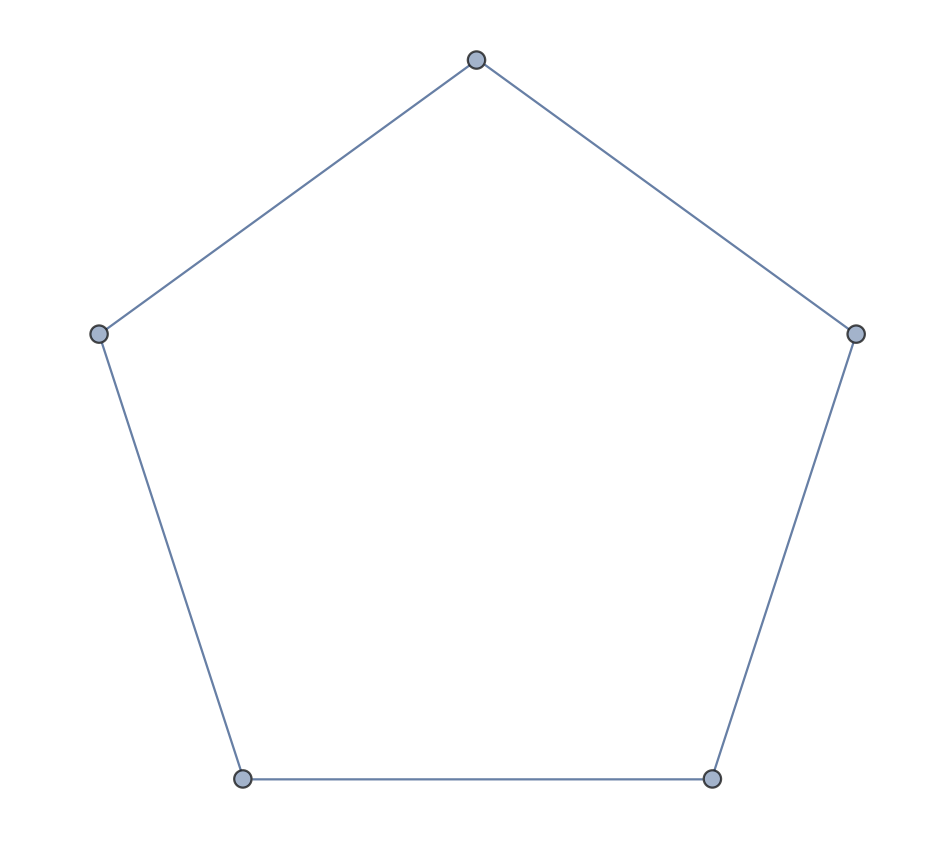
\includegraphics[width=50mm]{./figures/chapter1/cycle} &   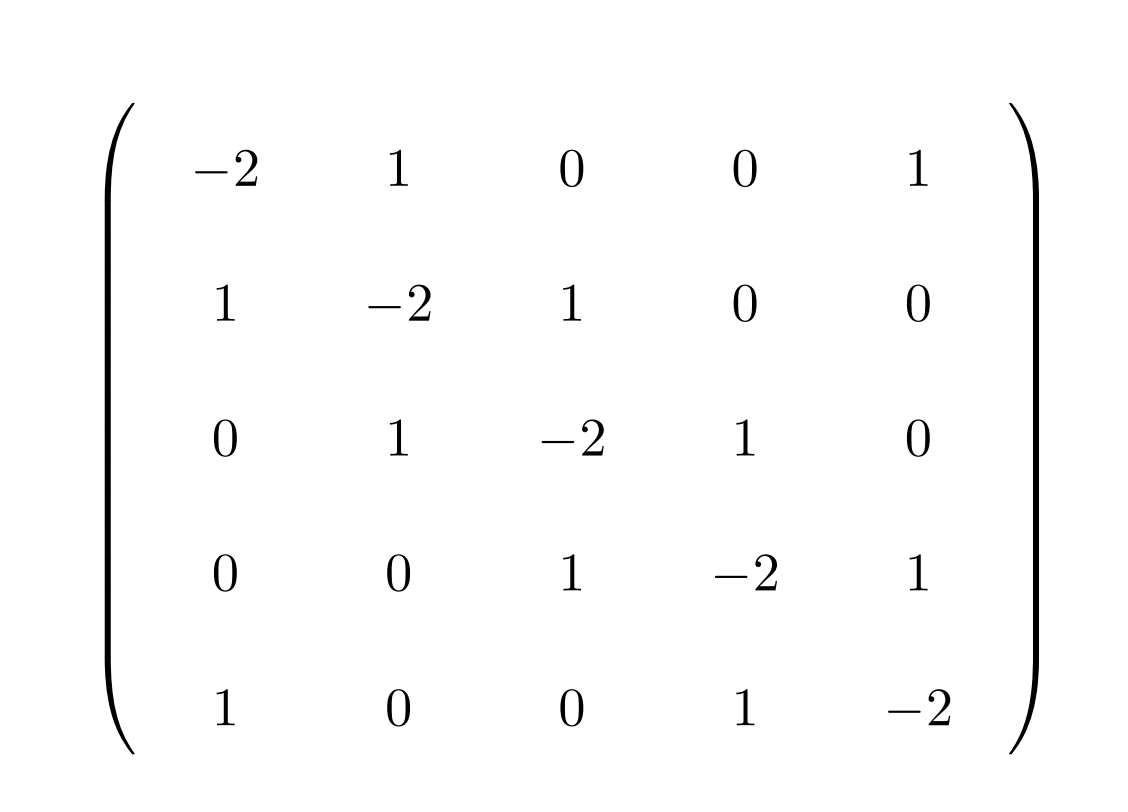
\includegraphics[width=50mm]{./figures/chapter1/cycleL} \\
          (a)  & (b) \\[6pt]
          \end{tabular}
          \caption[Pictorial representation of a cycle graph, and matricial representation for the Laplacian]{Pictorial representation of a cycle graph with 5 nodes (a), and the matricial representation for the Laplacian of Cy(5)}
        \end{figure}
    \vspace{-0.7cm}
    \subsection{Complete Graph}
    %\addcontentsline{toc}{subsection}{Complete Graph}
        A graph with N vertices is said to be complete if every node is adjacent to all the other N-1 nodes, thus representing a finite bidimensional structure. Its Laplacian matrix is given by:
        \begin{equation}
            L = (N-1)\sum_{j=1}^{N}\ket{j}\bra{j} - \sum_{k\neq j}\ket{j}\bra{k}
        \end{equation}
        A pictorial representation of a complete graph is given in figure. We will refere to this kind of graph with $C(N)$.
        \begin{figure}[hb]
          \centering
          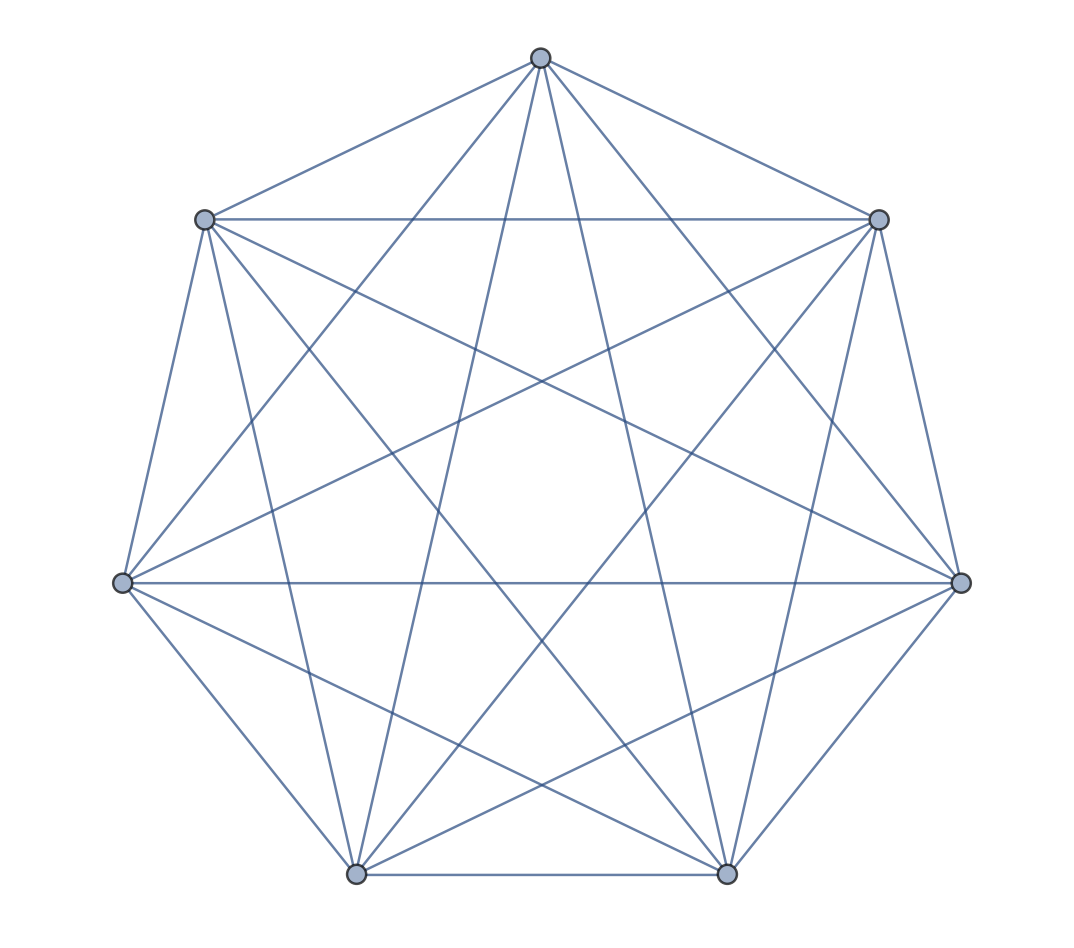
\includegraphics[width=50mm]{./figures/chapter1/complete}
          \caption[Pictorial representation of a complete graph]{Pictorial representation of a complete graph with N=7}
        \end{figure}

\section{Quantum Walks}
The continous time quantum walk (CTQW) is the direct analougue of the classical continous time random walk (CTRW). We begin by considering the classical one, expanding later on the quantum mechanical counterpart. \nocite{Mulken2011} \\
Let $j$ be a note of a graph $G$ and the initial node, such date the initial state of the system is $\ket{j}$. Then, we denote the transition probability of the walker to go from node j to a node k in a time t with $p_{k,j}(t)$. The state after time $t$ is given by $\ket{j;t}$, such that the overlap with node $k$ is $\braket{k|j;t}=p_{j,k}(t)$. \\
The dynamics resulting in the state $\ket{j;t}$ follows from transition rates per unit time between two nodes. In particular these transition rates are the components of the so-called \textit{transfer matrix} $T$, namely $T_{ij}= \bra{k}T\ket{j}$ . If we assume a Markovian process, the following master equation defines the CTRW evolution:
\begin{equation}
  \frac{d}{dt}p_{k,j}(t) = \sum_{l}T_{kl}p_{l,j}(t)
  \label{rw_master}
\end{equation}
In the simplest case, where the transitions rates for all edges are equal, the transfer matrix is closely related to the Laplacian matrix through :
\begin{equation}
  T = -\gamma L
\end{equation}
where $\gamma$ is the transition rate. The solution of \cref{rw_master}, along with the normalization constrains $\sum_{k=1}^{N}p_{k,j}(t) = 1 \hspace{3pt} \forall t$, is given by
\begin{equation}
  p_{ij}(t)= \braket{k|e^{Tt}|j} = \braket{k|e^{-\gamma At}|j}
\end{equation}
Turning to quantum mechanics the evolution of any physical system obeys the Schroedinger equation, and QWs represent no exception. The dynamics of the CTQW is governed by a specific Hamiltonian $H$, such that the Schroedinger equation for the transition \textit{amplitudes} $\alpha_{i,j}(t)$ is given by
\begin{equation}
  \frac{d}{dt}\alpha_{i,j}(t) = -i \sum_{l}H_{k,l}\alpha_{l,j}(t)
\end{equation}
where $H$ is the Hamiltonian of the systemm, and for semplicity we assume $\hbar = 1$. The formal solution of such differential equation is similarly to the CTRW given by
\begin{equation}
  \alpha_{l,j}(t) = \braket{k|e^{-iHt}|j}
  \label{qw_master}
\end{equation}
where $e^{-iHt}$ is the quantum mechanical time-evolution operator. We immediately notice the similar structure of equations (\ref{rw_master}) and (\ref{qw_master}), with the only difference apart from the imaginary unit  that the first is a differential equation for transition probabilities while the latter allows to compute transition amplitudes. The similarity is further pushed bu Farhi and Gutmann in 1998 \cite{Childs2001}, when they proposed to identify the Hamiltonian $H$ of the system with the negative of the classical transfer matrix $T$, which as we've seen previously is the Laplacian of the graph \footnote{Please note that in this particular scenario the transition amplitude $\gamma$ is set to one.}:
\begin{equation}
  H = -T = L
  \label{qw_hamiltonian}
\end{equation}
Therefore the Laplacian matrix completely determines the evolution of the quantum system as well as the classical scenario.



\section{Grover's Quantum Search}
In 1997 Lov K. Grover addressed the search problem through a quantum mechanical algorithm \cite{Grover1997}. The search problem itself can be formulated in the following way: given an unsorted database containing N items, with only one satisfing a given condition, that one item has to be retrieved. Once an item is examined, it's possible to determine whether it represents the solution or not in just one step.
Classically, the most efficient algorithm has to check each and every item in the database individually. If the item checked satisfies the condition the process stops, otherwise it will continue to examine the remaining items until the solution is find. On average, the algorithm will have to check $0.5N$ items before finding the desired one.\\On the other hand, Grover's quantum mechanical approach takes advantage of the \textit{superposition} of states in a quantum system, and by having the input and output in such superposition can find the desired objects in $O(\sqrt{N})$ \textit{quantum mechanical steps}, instead of $O(N)$ classical steps. As we shall see later, this quantum mechanicals steps consists of an elementary unitary operation. \\

Let's look at the algorithm to the quantum search problem more in detail, in particular setting the stage for the search algorithm in terms of an \textit{oracle}, which plays a central role in Grover's search and throughout the entire thesis. Additionally, this allows us to present a very general description of the search procedure, and a geometric way to visualize its action \cite{Nielsen2000}. \\
Suppose we want to search through a search space of $N$ elements, and let's consider the indices of such elements - instead of the actual elements - which clearly are numbers from 0 to $N-1$. In order to easily store the index in $n$ bits we consider $N=2^n$, and assume that the particular search problem has $M$ solutions, with $1\leq M\leq N$. We can now easily represent one instance of the search, i.e. checking if the item satisfies a particular condition, with a function $f(x)$, where $x$ is the index integer ranging from 0 to $N-1$. The function is such that if $x$ represents the solution to the search problem $f(x)=1$, and $f(x)=0$ if not a solution.




\section{Search by Quantum Walks}
The search problem first introduced by Grover can be reformulated in terms of search based on a continous-time quantum walk on a graph \cite{Childs2004}. \\In order to do so we need to modify the quantum walk hamiltonian of \cref{qw_hamiltonian} so that the vertex $\ket{w}$ is somewhat special. Therefore, an \textit{oracle hamiltonian} is introduced:
\begin{equation}
  H_w = -|w\rangle\langle w|
\end{equation}
that has energy zero for all but the vertex $|w\rangle$ for which it has enenergy $-1$. Therefore the Grover problem becomes finding the ground state of this hamiltonian. \\To implement the search we consider the Hamiltonian
\begin{equation}
  H = \gamma L + H_w = \gamma L -|w\rangle\langle w|
\end{equation}
where L is the laplacian of the graph $G$, that as we've seen in section? governs the evolution of the quantum walk.\\
The quantum search routine works as following:
\begin{itemize}
  \item we consider the balanced superposition of all possible states, namely
  \begin{equation}
    |s\rangle = \frac{1}{\sqrt{N}}\sum_j|j\rangle
  \end{equation}

  \item we run the quantum walk for a time $t_f$ and find the corrisponding evolved state using the hamiltonian $H$
  \begin{equation}
  |\psi(t_f)\rangle = U(t_f)|s\rangle  = \mbox{exp}\Big\{-\frac{i}{\hbar}Ht_f\Big\}|s\rangle
  \end{equation}
  (Note that this evolution is valid only for time-independent hamiltonians.)

  \item we then measure the state onto the target $|w\rangle$ and find the corrisponding probability
  \begin{equation}
    p = |\langle w|\psi(t_f)\rangle|^2
  \end{equation}

\end{itemize}
\noindent
The objective is to find the optimal value of $\gamma$ so that the success probability $|\braket{w|\psi(t_f)}|^2$ is as close as possible to 1 for the smallest $t_f$. \\ \\
We can turn our attention on trying to understand why we should expect this algorithm to give a success probability for some values of $\gamma, t_f$. To motivate this we need to frame the problem in terms of Hamiltonian spectrum. In particular we look at the two extremes, namely $\gamma\rightarrow\infty$ and $\gamma\rightarrow 0$.
\begin{itemize}
  \item as $\gamma\rightarrow\infty$ the contribution of $H_w$ is somewhat negligible, to the point that the ground state of $H$ is $\ket{s}$\footnote{Note that regardless of the graph topology considered, $\ket{s}$ is the ground state of the Laplacian, with $L\ket{s} = 0$.}
  \item on the other hand, if $\gamma\rightarrow 0$ the contribution of the Laplacian to the overall Hamiltonian $H$ disappears and thus the ground state of $H$ is close to $\ket{w}$
\end{itemize}
We expect that for some intermediate $\gamma$ the ground state will transition from $\ket{w}$ to $\ket{s}$ and thus could have substantial overlap on both for a certain value of $\gamma$. Additionally, if the first excited states have substantial overlap at such values of $\gamma$, then the Hamiltonian will drive transitions between two states, thus rotating the state from $\ket{s}$ to one with substantial overlap with $\ket{w}$, giving the success probability that we previously talked about. In particular this transition will happen in a time that dependes on the Hamiltonian eigenvalues separation between the first and ground state, namely $1/(E_1-E_0)$. \\ \\This is a good description of the algorithm if the dimension of the graph is sufficiently high.  However, if we consider a $d$-dimensional lattice with $d$ independent of $N$ we still see that for a critical value of $\gamma$ the state switches from the ground state to the first excited state, but for $d<4$ the $\ket{w}$ state does not have substantial overlap on the ground and fist excited state, thus the algorithm does not work. \\
\textbf{Comments on the oracle $H_w$}: The oracle introduce in this fashion is exactly the continous-time version of the reflection $R_w$ in Grover's algorithm \cite{Wong2016} because by itself it only evolves the marked vertex $\ket{w}$ by a phase
\begin{equation}
  e^{-i\ket{w}\bra{w}t}\ket{w} = e^{-it}\ket{w}
\end{equation}
while leaving the other vertices unchanced, thus making this the continous-time version of a yes/no oracle.

\subsection{Search on Complete Graph}
We now look at the complete graph which can be thought of having dimension proportional to N and represents the simples example of the quantum walk search application \cite{Childs2004}. \\We begin by noticing that adding a multiple of the identity matrix to the Laplacian only contributes a global unobservable phase. We add $-NI$ so that:
\begin{equation}
  L - NI = N\ket{s}\bra{s}
\end{equation}
This gives us the following Hamiltonian:
\begin{equation}
  H = -\gamma N \ket{s}\bra{s} - \ket{w}\bra{w}
\end{equation}
In particular we know that this hamiltonian acts non-trivially in a two dimensional subspace spanned by $\ket{s}$ and $\ket{w}$, thus making it stright-forward to compute its spectrum. If we use the $\{\ket{w}, \ket{r}\}$ basis, the hamiltonian can be expressed in the following way:
\begin{equation}
  H = \frac{-1}{N} \begin{pmatrix} N+1 & \sqrt{N-1}\\ \sqrt{N-1} & N-1 \end{pmatrix}
\end{equation}
Applying the time-evolution operator to the initial state $\ket{s}$, the system at time $t$ will be
\begin{equation}
  \ket{\psi(t)} = e^{it}
  \begin{pmatrix}
  \frac{1}{\sqrt{N}}\cos(\frac{t}{\sqrt{N}}) +i\sin(\frac{t}{\sqrt{N}})\\
  \sqrt{\frac{N-1}{N}}\cos(\frac{t}{\sqrt{N}})
  \end{pmatrix}
\end{equation}
and for $t=\pi\sqrt{N}/2$ the system reaches a success probability of 1, namely
\begin{equation}
  p = \Big|\braket{w|\psi(t)}\Big|^2_{t=\pi\sqrt{N}/2} = \Big|\braket{w |  ie^{it}w}\Big|^2 = 1
\end{equation}
recalling that in the 2-dimensional subspace $w = (0,1)$. Thus the walk rotates the state from $\ket{s}$ to $\ket{w}$ in $O(\sqrt{N})$.

\section{Search by Adiabatic Evolution}
We now address the computation by adiabatic evolution firstly introduced by Farhi et al., that takes advantage of the adiabatic theorem to find the solution of a computational problem \cite{Farhi2000}. We begin by looking at the \textit{adiabatic theorem} and its implication. Then, an overview of the adiabatic implementation of the algorithm for solving the unstructured search problem is given which has a time scaling of $O(N)$. Lastly, we see how applying the adiabatic theorem \textit{locally} can lead to a time of order $O(\sqrt{N})$ which is optimal.

    \subsection{Adiabatic Theorem}
    A quantum system evolves according to the Schroedinger equation
    \begin{equation}
        i\frac{d}{dt}|\psi(t)\rangle = H(t)|\psi(t)\rangle
    \end{equation}
    and defining the instantaneous eigenstates and eigenvalues of H(t) by
    \begin{equation}
        H(t)|l;t\rangle = E_l(t)|l;t\rangle
    \end{equation}
    such that $E_0(t) \geq E_1(t) \geq ... \geq E_{N-1}(t)$. \\
    The adiabatic theorem states that if the gap between the two lowest energy levels, $E_{1}(t) - E_{0}(t) > 0$, is stritcly greater than zero then for $T\rightarrow \infty$ the probability of being in the ground state is equal to one, namely
    \begin{equation}
        \lim_{T \to \infty} |\langle l=0;t = T | \psi(T)\rangle| = 1
    \end{equation}
    This means that if the system is chosen to evolve at a slow enough rate, the instantaneous hamiltonian will remain in the ground state throught the evolution. It is useful to consider a smooth one-parameter hamiltonian $H(s)$ such that $s=t/T$, with $t \in [0,T]$ so that $s \in [0,1]$.
    Let's now define the energy minimum gap by
    \begin{equation}
        g_{min} = \min_{0 \leq s \leq 1} (E_1(s)-E_0(s))
    \end{equation}
    In addition we can find a time lower bound $T^*$ such that for $T\gg T^{*}$ the probability is arbitrarily close to 1, in detail
    \begin{equation}
        T \gg \frac{\varepsilon}{g^{2}_{min}}
    \end{equation}
    where
    \begin{equation}
        \varepsilon = \max_{0 \leq s \leq 1} \Big| \Big\langle l=1;s\Big| \frac{dH(s)}{dt} \Big| l=0;s\Big\rangle\Big|
    \end{equation}

    Let's now discuss how to take advantage of the adiabatic theorem introducting the usual way in which the adiabatic evolution is implemented. It is often presented a problem hamiltonian $H_P$ whose ground state is not so straight forward to find; on the other hand we can prepare the system in abeginning hamiltonian $H_B$ whose ground state is known. The problem hamiltonian encodes the solution of the problem, while the beginning hamiltonian is a tool for easily preparing the state to be evolved. The adiabatic implementation then consists, assuming that the ground state of $H_P$ is unique, in having a time dependent hamiltonian $H(s)$ such that
    \begin{equation}
        H(s) = (1-s)H_B + s H_P
    \end{equation}
    In this way we can prepare for $s=0$ the system in $H_B$ and let it evolve so that for $s=1$ it reaches $H_P$. Thanks to the adiabatic theorem, if it's made to evolve sufficiently slowly we will find ourself in the ground state of the problem hamiltonian, which is exactly the solution.

    \subsection{Global adiabatic evolution}
    Let's now apply what just seen to the unsorted search problem \cite{Roland2002}. As done in Section? we consider an unsorted database of $N$ elements such that $N=2^n$, so that the elements in this particular basis can be written as $\ket{i}$, with $i=0,...,N-1$. The marked state can be then denoted as $\ket{w}$, and we begin by considering the initial state as the superposition of all the elements $\ket{i}$:
    \begin{equation}
      \ket{\psi_0}=\frac{1}{\sqrt{N}}\sum_{i=1}^{N-1}\ket{i}
    \end{equation}
    With this in mind we design two particular Hamiltonians $H_0$ and $H_w$ such that $\ket{\psi_0}$ is the ground state of the first while $\ket{w}$ is the ground state of the latter:
    \begin{equation}
      H_0 = I- \ket{\psi_0}\bra{\psi_0}
    \end{equation}
    \vspace{-1cm}
    \begin{equation}
      H_w = I- \ket{w}\bra{w}
    \end{equation}
    The time-dependent Hamiltonian follows from the adiabatic implementation discussed in Section?, where $H_0$ is the beginning hamiltonian while $H_w$ is the problem hamiltonian. It thus consists in a linear interpolation between $H_0$ and $H_w$:
    \begin{equation}
      H(t) = (1-s)H_0 + sH_w
    \end{equation}
    where $s=t/T$ is the linear interpolating schedule.\\ \\
    The search routine runs as usual, beginning with preparing the system in the state $\ket{\psi(0)}=\ket{\psi_0}$ and then applying the Hamiltonian $H(t)$ for a time $T$. We're interested in finding the time-dependent condition such that the system evolves sufficiently slowly, allowing us to find the solution $\ket{w}$ with high probability. First, we determine the quantity $\braket{\frac{dH}{dt}}$:
    \begin{equation}
      \braket{\frac{dH}{dt}}_{0,1} = \frac{ds}{dt}\braket{\frac{dH}{ds}}_{0,1} = \frac{1}{T}\braket{\frac{dH}{ds}}_{0,1}
    \end{equation}
    We then find the eigenvalues of the Hamiltonian and determine the separation $g$ between the ground state and first excited one, namely $E_1$ and $E_0$, as a function of the interpolating schedule s:
    \begin{equation}
      g=\sqrt{1-4\frac{N-1}{N}s(1-s)}
      \label{separation}
    \end{equation}
    We're interested in the minimum gap $g_{\min}$ which is found for $s=1/2$. Additionally we find that $\big|\braket{\frac{dH}{ds}}_{0,1}\big| \leq 1$, therefore Eq? becomes:
    \begin{equation}
      \frac{\big|\braket{\frac{dH}{ds}}_{0,1}\big|}{g_{\min}^2} \leq \varepsilon
      \label{adiabatic_condition}
    \end{equation}
    so that the adiabatic condition is verified, and thus the hamiltonian stays in the ground state at all times, provided that $T\geq N/\varepsilon$. Therefore the computation time is of order $N$, showing no speed up compared to the classical search.

    \subsection{Local adiabatic evolution}
    Roland and Cerf showed that the adiabatic evolution can be improved by applying the adiabatic condition of \cref{adiabatic_condition} locally instead of globally \cite{Roland2002}. If we look at the plot of the separation $g$ we see that the adiabatic condition is critical only for $s=1/2$ where it reaches its minimum.
    \begin{figure}[h]
      \centering
      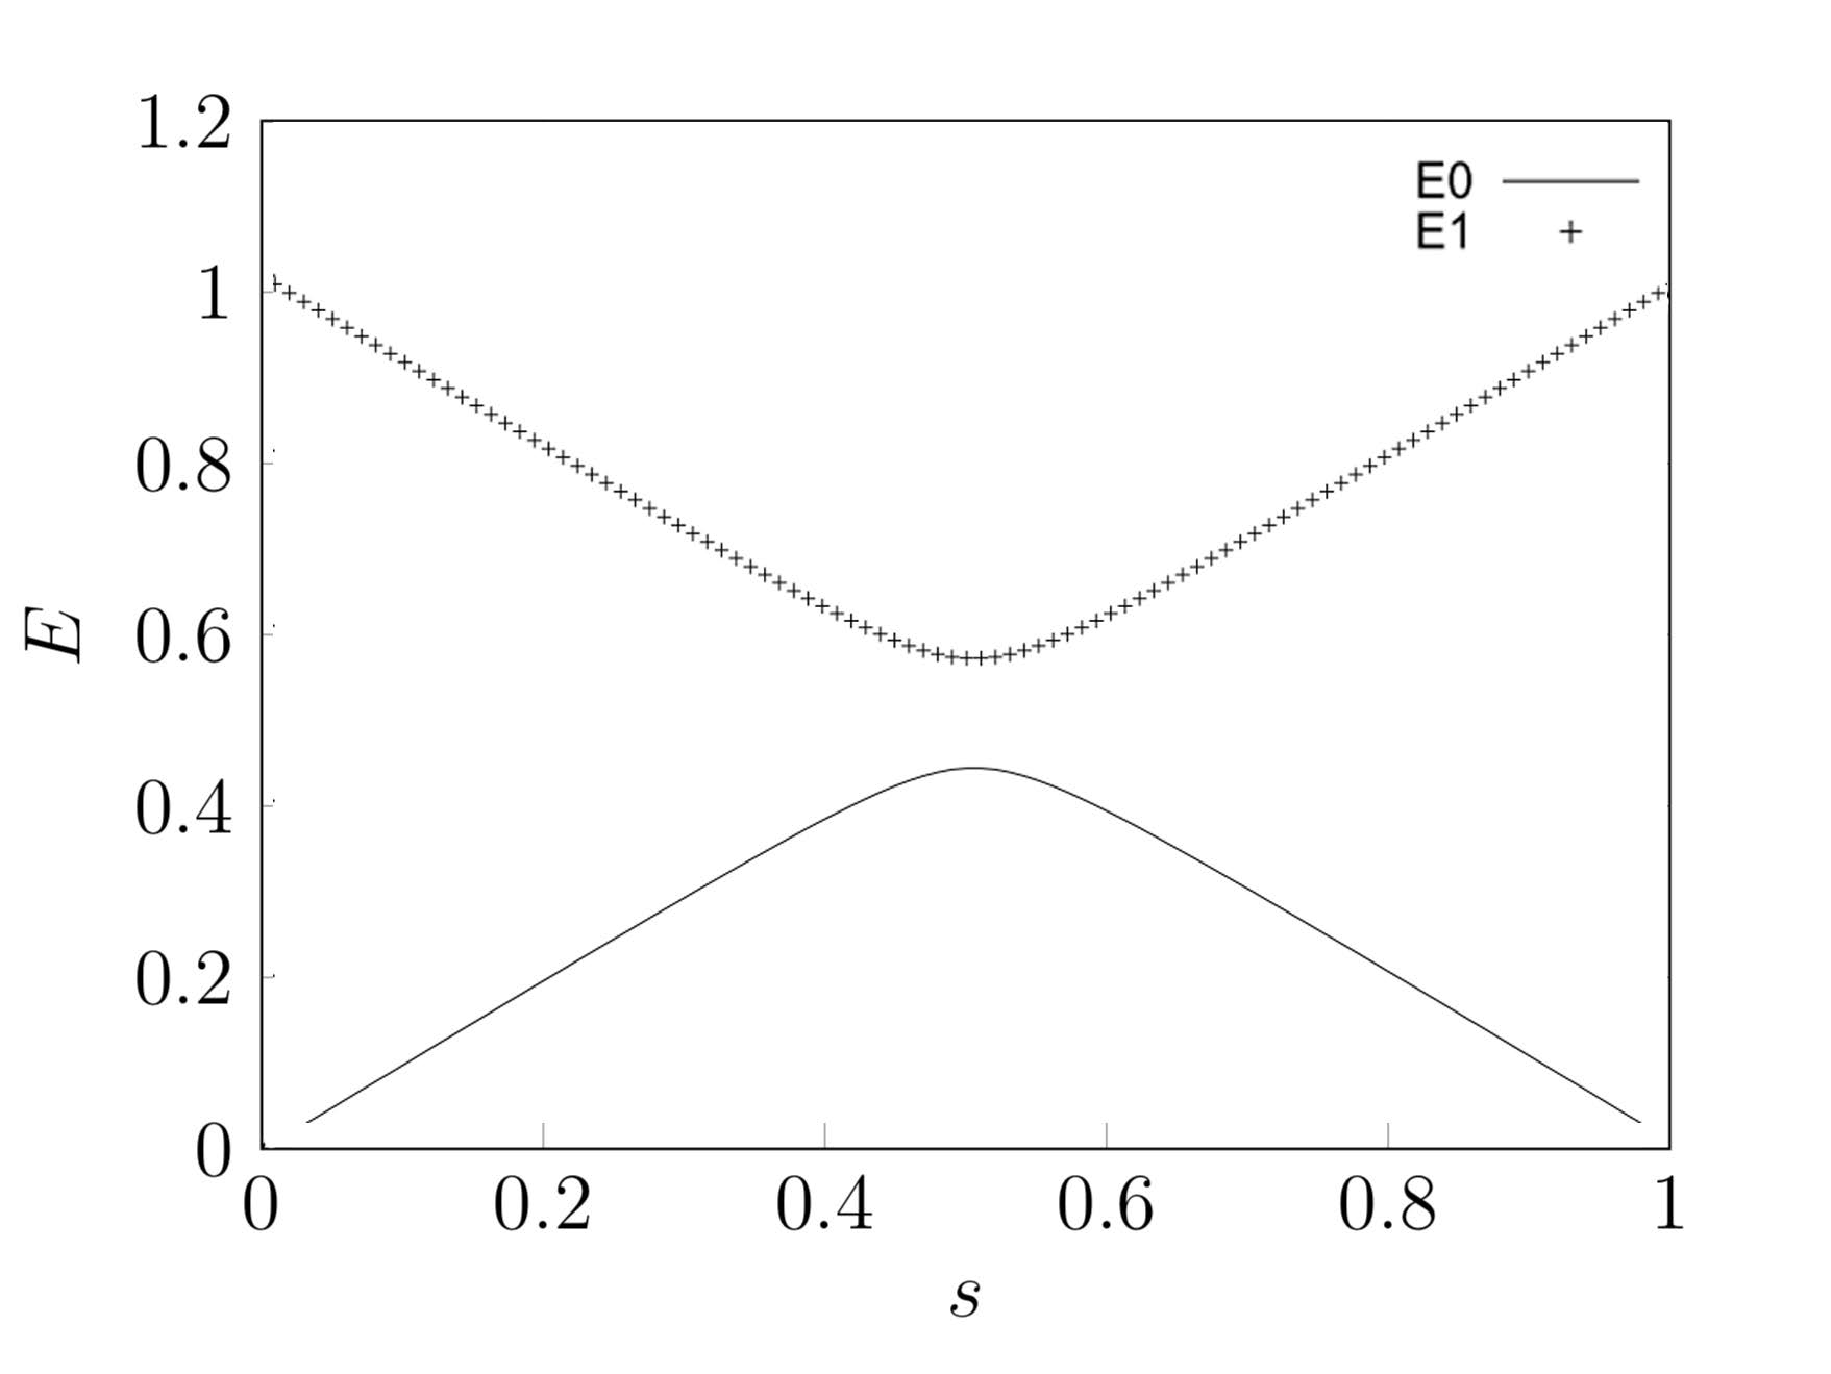
\includegraphics[width=80mm]{figures/chapter1/separation}
      \caption[Eigenvalue separation of the time-dependent Hamiltonian $H(s)$ as a function of the reduced time $s$, for N=64]{Eigenvalue separation of the time-dependent Hamiltonian $H(s)$ as a function of the reduced time $s$, for N=64. \textit{Figure from Roland and Cerf} \cite{Roland2002}}
      \label{separation_figure}
    \end{figure}
    At the beginning and at the end of the evolution the separation is large enough so that the adiabatic condition and thus the time necessary for the system to evolve adiabatically is small, allowing for better time scaling. The improvement comes in the form of the interpolating schedule, following the idea that it should be steeper for large separation $g$ and flatter (more than linear) for small separation around $s=1/2$. Let's see how can this be done. \\ \\
    We divide the interval $[0,t_f]$ into infinitesimal intervals $dt$ and adapt the evolution rate $\frac{ds}{dt}$ to the local adabatic condition. In this way we can find the optimal $s(t)$, with boundary conditions $s(0)=0$ and $s(t_f)=1$. We find the new adiabatic condition for all time $t$:
    \begin{equation}
      \Big|\frac{ds}{dt}\Big|\leq\varepsilon\frac{g^2(t)}{\big|\braket{\frac{dH}{ds}}_{0,1}\big|}
    \end{equation}
    Using \cref{separation} and $\big|\braket{\frac{dH}{ds}}_{0,1}\big| \leq 1$ and Hamiltonian is chosen to evolve with the interpolating schedule that is solution of the following differential equation (with $\varepsilon<<1$):
    \begin{equation}
      \frac{ds}{dt} = \varepsilon g^2(t) = \varepsilon\Big[1-4\frac{N-1}{N}s(1-s)\Big]
    \end{equation}
    After integration we get the following
    \begin{equation}
      t =\frac{1}{2\varepsilon}\frac{N}{\sqrt{N-1}}\Big[\arctan\big(\sqrt{N-1}(2s-1)\big) + \arctan{\sqrt{N-1}}\Big]
    \end{equation}
    By inverting we find the interpolating schedule $s(t)$ as can be seen in \cref{interpolating_schedule}. In order to determine the computation time of this algorithm. To do so we evaluate $s=1$ and in the approximation that $N>>1$ we get:
    \begin{equation}
      T = \frac{\pi}{2\varepsilon}\sqrt{N}
    \end{equation}
    which represents a great improvement on Eq?. Indeed we have a quadratic speed up compared to the global adiabatic evolution, and thus this algorithm can be seen as the adiabatic implementation of the Grover's search algorithm.
    \begin{figure}[h]
      \centering
      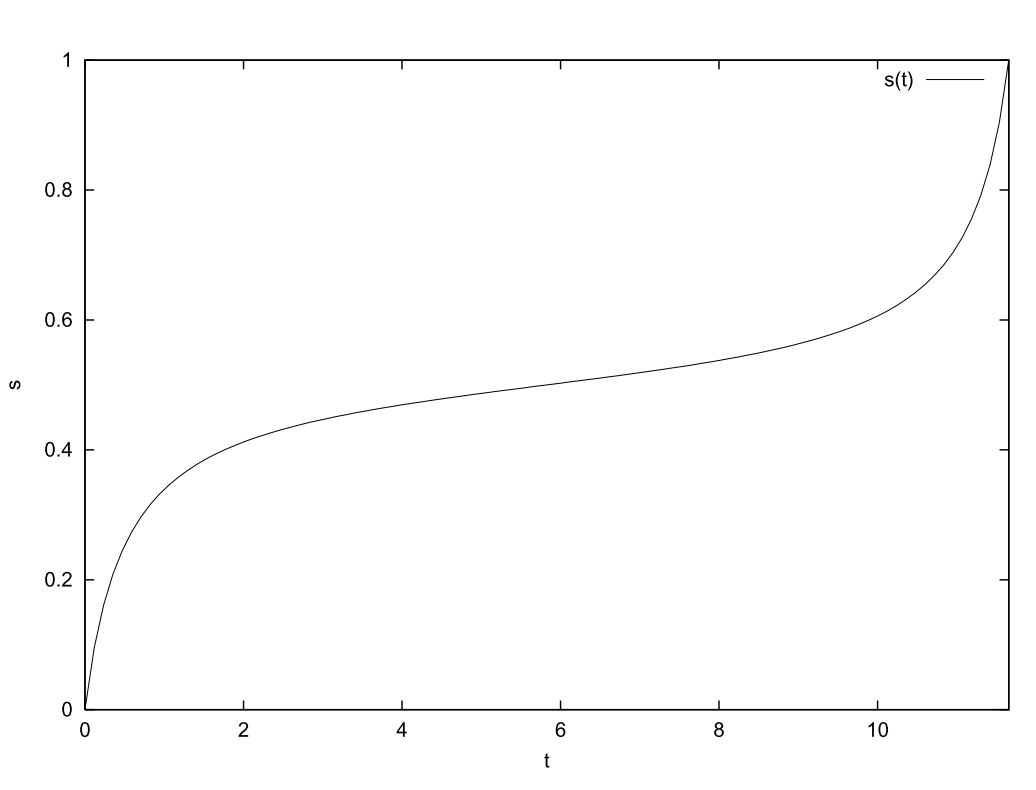
\includegraphics[width=80mm]{figures/chapter1/interpolating_schedule}
      \caption[Eigenvalue separation of the time-dependent Hamiltonian $H(s)$ as a function of the reduced time $s$, for N=64]{Eigenvalue separation of the time-dependent Hamiltonian $H(s)$ as a function of the reduced time $s$, for N=64. \textit{Figure from Roland and Cerf} \cite{Roland2002}}
      \label{interpolating_schedule}
    \end{figure}



\section{Impossibility of Adiabatic Quantum Walks}
In this section we show that an \textit{adiabatic quantum walks} based search algorithm cannot be implemented with the usual Grover's oracle and requires a more sophisticated structure. This section, based on a paper by Wong et al. \cite{Wong2016}, sets the basis on which our work takes place. \\ \\
In the previous sections we discussed Grover's original discrete-time search algorithm, Farhi and Gutmann's quantum walk analogue and Roland and Cerf's adiabatic analogue. Throught the discussion we analysized the systems in a 2-dimensional subspace spanned by $\big\{\ket{w}, \ket{r}\big\}$. We this in mind we can visualize the evolution of the quantum algorithm on the two dimensional Bloch sphere and compare the path taken by each different approach. In particular we notice that the original Grover's algorithm and the Roland and Cerf's local adiabatic evolution follow the same path on the $xz$-plane since they both always have real coefficients, as can be seen in fig? (a) and (b) respectively. On the other hand the quantum walk formulation of Farhi and Gutmann has an unmeasurable complex phase thus it evolves on a different path on the $yz$-plane of Fig

\begin{figure}[h]
     \centering
     \subfloat[Grover]{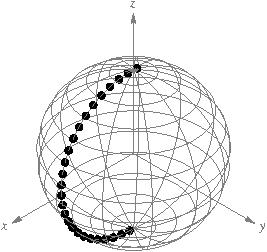
\includegraphics{figures/chapter1/blochsphere_Grover}\label{fig:blochsphere_Grover}}
     \subfloat[Roland-Cerf]{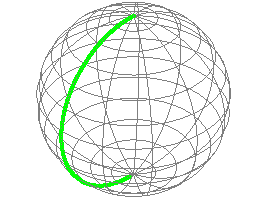
\includegraphics{figures/chapter1/blochsphere_RC}\label{fig:blochsphere_RC}}
     \subfloat[Farhi-Gutmann]{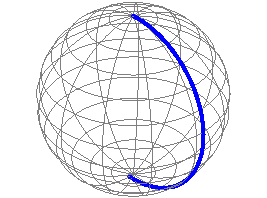
\includegraphics{figures/chapter1/blochsphere_FG}\label{fig:blochsphere_FG}}
     \caption{Path evolution \cite{Wong2016} dfjs hfdjsfh}
     \label{steady_state}
\end{figure}


%%%%%%%%%%%%%%%%%%%%%%
%%%%%%%%%%QUANTUM WALKS WITH TIME DEPENDENT HAMILTONIANS%%%%%%%
%%%%%%%%%%%%%%%%%%%%%%%
%\newpage
\thispagestyle{empty}
\chapter{Quantum Walks with Time-Dependent Hamiltonians}
The main purpose of this thesis is to study quantum walks with time dependent hamiltonians, focusing in particular on their application to the spatial search problem on graph. The general idea is trying to improve a time-independent implementation of quantum walks search using a time-dependent hamiltonian analogous to the one used in the adiabatic evolution. In order to determine whether this new approach produces successfull results we study two selected graph topology: the circular graph, for which the time-independent approach is not able to solve the search problem, and the complete graph for which the search problem is solved for both the time-independent and adiabatic evolution approaches. \\ We compare the two methods for the optimized-search, localization - which represents a search without needs to optimize the time - and a measure of robustness.

\section{Search with Time-Dependent Hamiltonian}
In Section? we discussed the use of quantum walks for the spatial search problem \cite{Childs2004} and the application to the complete graph where the search problem is solved. We then illustrated how the adiabatic theorem can be used to solve computational problems with an adiabatic evolution of a quantum system \cite{Farhi2000}. Efforts to combine the two approaches showed that the search problem can be solved only with structures stronger than the usual Grover's oracle \cite{Wong2016}, thus making an \textit{Adiabatic-Quantum-Walk-Search} impossible. However this leaves space to a merely time-dependent quantum walk search, that takes advantage of a time-dependent implementation similar to the adiabatic evolution but that is not bounded to the strict adiabatic-theorem conditions and the limitation of the standard Grover's oracle.


    \subsection{Time-Dependent Quantum Walk}
        Following from the adiabatic evolution discussed in the preliminaries, we consider a search hamiltonian that interpolates between an initial hamiltonian, i.e. the laplacian of the graph $L$, and the final oracle hamiltonian $H_w=\gamma\ket{w}\bra{w}$
          \begin{equation}
            H(s) = (1-s)L - s\gamma|w\rangle\langle w|
          \end{equation}
        where the interpolation schedule $s=s(t)$ goes from 0 to 1 as the time $t$ goes from 0 to the runtime $t_f$. \\ \\In order to find the evolved ground state of the beginning hamiltonian we need to determine the evolution operator that for a time-dependent hamiltonian is given by:
        \begin{equation}
          S(t,t_0) = \mbox{T} \mbox{exp} \frac{1}{i\hbar}\Big\{ \int_{t_0}^{t} dt' H(t')\Big\}
        \end{equation}
        where T is the time-ordering. Since we're only interested in the evolved state, having the exact evolution operator is somewhat irrelevant. Additionally for the circular graph - which represents the main topology studied in this thesis - the search hamiltonian does not show any particular properties making an analitical derivation of the operator not possible. We therefore proceed by solving the differential Schroedinger equation:
        \begin{equation}
          i\frac{d}{dt}|\psi(t)\rangle = H |\psi(t)\rangle
        \end{equation}
        Recalling that we're dealing with matrices and vectors in an N-dimensional Hilbert space, we solve N-differential equations of the form
        \begin{equation}
        \frac{d}{dt}|\psi_i(t)\rangle = \sum_jH_{ij}|\psi_i(t)\rangle
        \end{equation}
        with the boundary conditions $|\psi_i(0)\rangle = |\psi_i\rangle$.\\
        From a numerical point of view this approach is also much simpler than other direct methods of evaluating the evolution operator, such as the Dyson Series or Magnus Expansion.




    \subsection{Interpolating Schedule s(t)}
        As pointed by Wong the interpolating schedule s(t) plays a crucial role in the evolution of the system and in the overall scaling of the algorithm.
        The original adiabatic evolution by Farhi and Gutmann. \cite{Farhi2000} uses a linear interpolating schedule defined as $s(t) = \frac{t}{t_f}$. Ronald and Cerf show that in order to obtain a quadratic speedup for the complete graph a non linear schedule is essential \cite{Roland2002}\cite{Morley2018}.

        Thus, from a linear interpolating schedule we begin considering, somewhat naively, quadratic and cubic schedules:
        \begin{equation}
          s(t) = \sqrt{\frac{t}{t_f}} \hspace{30pt} s(t) = \sqrt[3]{\frac{t}{t_f}}
        \end{equation}
        We then consider the interpolating schedule analitically derived by Ronald and Cerf for the unstructured search (complete graph) given by :
        \begin{equation}
            t = \frac{1}{2\epsilon}\frac{N}{\sqrt{N-1}}\Big[\mbox{arctan}\big(\sqrt{N-1}(2s-1)\big) + \mbox{arctan}\sqrt{N-1}\Big]
        \end{equation}
        By inverting the function, $s(t)$ is obtained as plotted in \cref{cerf}(a) \\
        The shape of this interpolating schedule comes from the gap $g(s)$ between the lowest two eigenvalues, changing faster when the gap is large, while it evolves slower when the gap is small. We therefore take these key aspects of $s(t)$ - derived for the unstructured search - an consider a similar interpolating schedule defined as follow
        \begin{equation}
            s(t) = \frac{1}{2}(2(x-1)^{3}+1)
        \end{equation}
        \begin{figure}[ht]
          \centering
          \begin{tabular}{cc}
            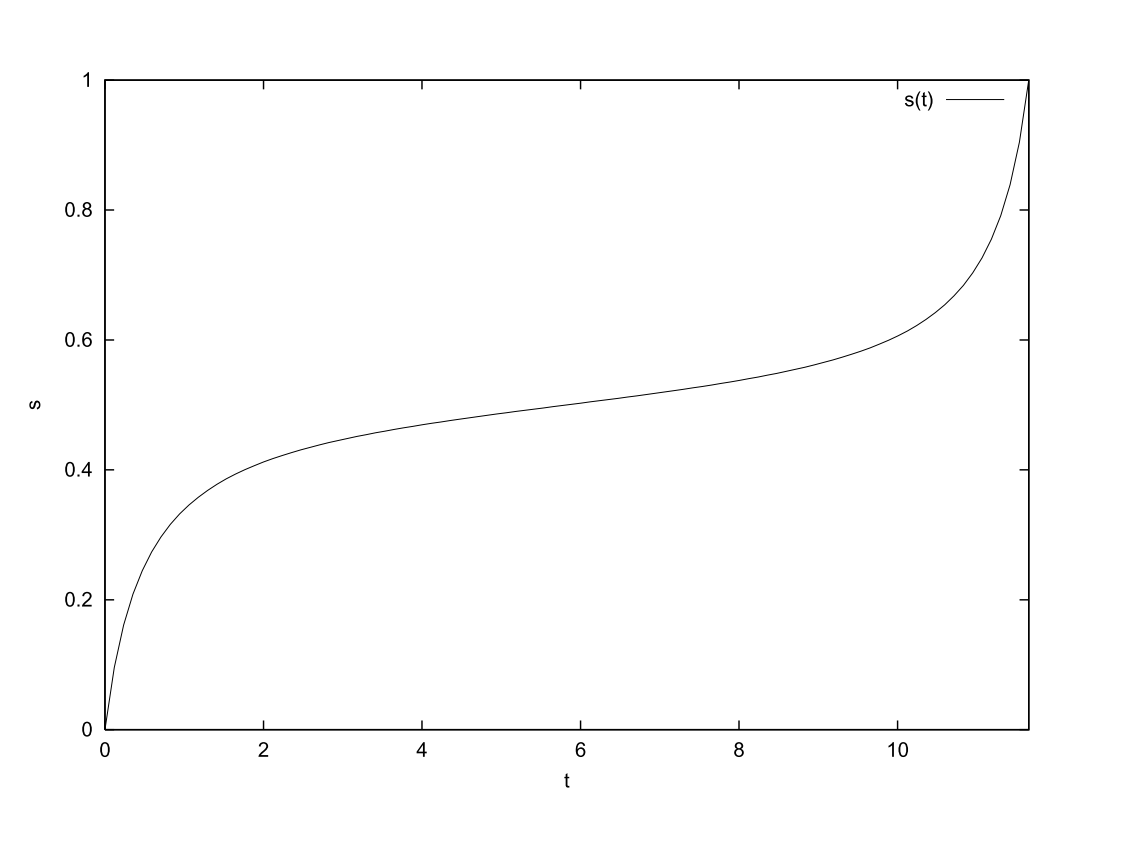
\includegraphics[width=75mm]{./figures/interpolating_schedules/cerf} &   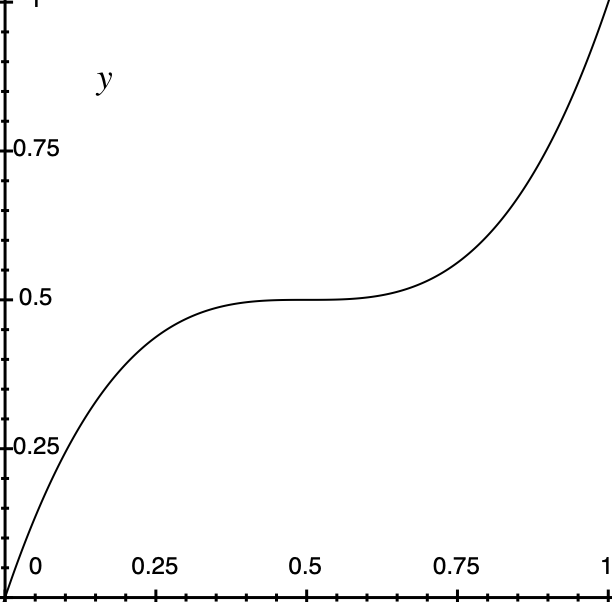
\includegraphics[width=45mm]{./figures/interpolating_schedules/our_cerf} \\
          (a) Original Ronald-Cerf & (b) Ronald-Cerf like\\[6pt]
          \end{tabular}
          \caption[Ronald and Cerf's interpolating schedules for the unstructured search and our non-linear schedule]{\textbf{Ronald and Cerf's interpolating schedule (a) and our Ronald-Cerf like schedule (b).} These figures show the difference between the original interpolating schedule derived by Ronald and Cerf for the unstructured search (left) and our Ronald-Cerf like schedule(right). Although quite different we study the effects of this particular non-linear interpolating schedule and compare it with the linear one used by Farhi and Gutmann \cite{Farhi2000}.}
          \label{cerf}
        \end{figure}

        \subsection{Multiple Runs for One Search}
        To give a complete picture of the usefulness of the time-depedent approach, we consider the possibility of repeating the search multiple times. If the probability at which the solution is found is $p=1$ the search is perfect and the problem is solved. However, if the proabability is less than one, i.e. imperfect search, the problem can be solved by searching multiple times . Since the results of the search are checked independently, a single successfull search is sufficient, and this kind of routine is efficient as long as the probability $\big|\langle\psi(t_f)| w\rangle\big|^2$ is greater than $1/poly(N)$ (where N is the dimension of the graph) \cite{Morley2018}.

        Repeating the search multiple times does however come at a cost. It is indeed necessary to take into account for a non-zero \textit{initialization} time $t_{init}$ to prepare the system in the correct state as well a physical time for the measurement. Therefore, computing multiple searches with small $t_f$ becomes less efficient than less searches with larger $t_f$, where the quantity $t_{init}$ makes a lesser contribution to the overall $t_f$. Clearly this consideration is particularly relevant for increasing graph size.

\section{Selected Topology: Circular and Complete Graph}
    Throughout our analysis we will focus the attention on two selected graph topology, the ring graph (R) and the complete graph (C). \\

    As previously discussed in Section? the \textbf{complete graph} represents the best case scenario since it has been shown to solve the search problem both for the standard time-independent quantum walk approach \cite{Childs2004} and the local adiabatic evolution \cite{Roland2002}, with a quadratic speed up. An adiabatic implementation of the quantum walk search does not work with the usual Grover's oracle requiring a more elaborate structure \cite{Wong2016}, however as we shall later see a merely time-dependent approach might give promising results in terms of robustness.  \\

    The \textbf{circular graph} on the other hand is not able to solve the search problem with the time-independent approach, and can give some interesting insights with the application of the time-dependent quantum walk search.  \\

    The choice of graph topology is therefore based on the idea of giving results at either side of the spectrum of 2-dimensional graphs, trying to improve a non-working approach on one side, and get some interesting insights on an already perfect-search approach on the other.

\section{Characterization of the results: Search, Localization and Robustness}
    Firstly it's necessary to define what type of results we're looking for. We begin by shwoing the difference between \textbf{search} and \textbf{localization}. Then we introduce a (not-so-rigorous) measure for the \textbf{robustness} of the search algorithm.

    \subsection{Search vs Localization}
      Before looking at the results it's necessary to characterize two particular classes of results, the \textbf{search} and the \textbf{localization}, that help us decide whether the time-dependent approach does bring any advantages.
      \begin{itemize}
          \item the (optimized) \textbf{search} describes the usual search, namely the finding of the solution with high probability (possibly unitary) for the smallest time as possible. As previously mentioned we also take into account the possibility of repeating the search multiple times.
          \item the \textbf{localization} describes the finding of the solution with high probablity without the need to optimize the time. This description becomes necessary if we take into account the adiabatic nature of the time-dependent approach, that guarantees unitary probability for large enough $t_f$.
      \end{itemize}

    \subsection{Robustness}
        We've seen that the probability of a search problem depends on the time $t_f$ at which the quantum state is measured and the parameter $\gamma$. The optimal probability, i.e. highest possible, clearly is given by the optimal combination $t_f-\gamma$, and since the time $t_f$ should not be bound to errors give it's the time at which the state is measured, fluctuations in the probability are necessarily caused by fluctuations in the $\gamma$ parameter. \\
        Following from \cite{SH.HungS.Hietala2019} we define the \textbf{robustness} as quantitative measure representing the variation on the probability due to some perturbation/noise on $\gamma$.
        We begin by finding the optimal probability $P$, evaluated with the single or multiple run for one search approach. For the corresponding $(t_f,\gamma)$ combination we evaluate the robustness as follows:
        \begin{equation}
            R ^\pm = P(t_f, \gamma) - P(t_f, \gamma \pm \delta)
        \end{equation}
        where $\delta$ is some positive perturbation of the $\gamma$ parameter. As we shall later see this quantity is given in terms of some percentage of $\gamma$. To find a unique value for the robustness an average of $R^\pm$ is done:
        \begin{equation}
            R = \frac{R^++ R^-}{2}
        \end{equation}
        The quantity R should be positive, since the $(t_f,\gamma)$ combination should produce the highest probability possible. We also that the perturbation on the parameter has equal probability of being positive or negative, thus the average ponderates between these two possibilities. \\ \\It is necessary however to remember that the value $R$ does not have any absolute physical significance, but fits well for our specific scenario where the interest is focused on the comparison between two specific approaches. Therefore this quantity will be solely used to characterize a particular approach as \textbf{more} or \textbf{less robust}.

\section{Results for the Circular Graph}
We now address the results for the circular graph. We begin by computing benchmarks for the time-independent hamiltonian approach; this should give us a good starting point for the comparison. Then we consider the time-dependent hamiltonian and evaluate the necessary data. We compare the two approaches, beginning from the Localization, followed by the Search which requires the introduction of a new quantity that takes into account the possibility of doing multiple runs for one search. Lastly we study the robustness of the time-dependent approach and determine whether the newly introduced hamiltonian makes the search more robust than the time-independent search.

    \subsection{Time-Independent Benchmarks}
        The first step of the analysis is to compute time-independent benchmarks. We computed the probability over a time-beta grid, with $T\in[0,N]$ and $\gamma\in[0,2.5]$, where N is the dimension of the graph considered. An initial run of the probability distribution showed that the probability does not increase with time, thus the need to evaluate for $t_f$ greater than $T=N$ proved to be unnecessary. In addition Grover algorithm for the unstructured search (and the complete graph) scales $\sqrt{N}$ and the Farhi and Gutmann's adiabatic evolution scales like $N$, thus focusing on $T \leq N$ made much more sense. \textbf{Figure of probability distribution for sampled $\gamma$} \\
        Throughout the analysis we will consider graphs up to N = 71, with only odd dimensions which makes a easier oracle placement. Additional considerations and reasoning for the time-gamma grid can be found in Appendix A. \\


        To display the results in an intuitive way we used a heatmap plot, which gives a good idea on the probability distribution for varying combinations of $(T,\gamma)$:

          \begin{figure}[ht]
            \centering
            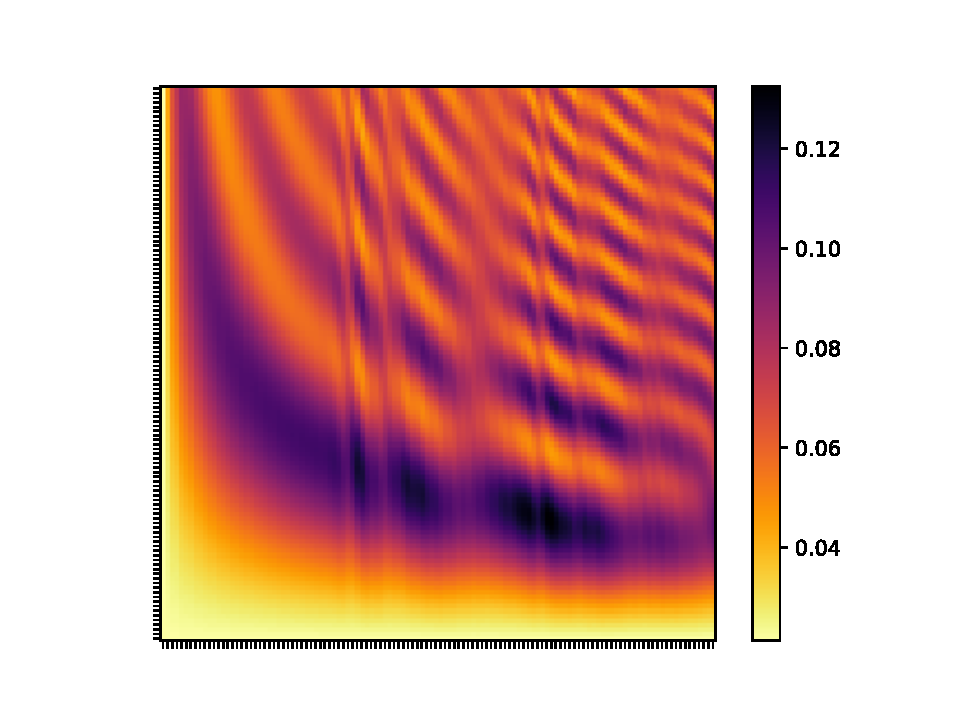
\includegraphics[width=9cm]{./figures/time_independent_benchmark_47}%
            \caption[Probability heatmap plot for the time-independent hamiltonian, N=47]{\textbf{Probability heatmap plot for the time-independent hamiltonian.} The figure shows the probability distribution for a circular graph of N=47 evaluated using the time-independent hamiltonian, providing thus the necessary benchmark. Note that dark color do not represent probabilities close to one, but only higher probability regions.}
          \end{figure}

        \subsubsection*{Comments on the probability distribution}
        From the heatmap plot we see that the probability distribution does not increase smoothly with increasing time, but shows peaks (dark regions) and valleys (lighter regions). Additionally dark regions are scattered throughout the grid and not necessarily for large $t_f$. We will later see that this is somewhat a weakness of the time-independent approach, since a small variation of the parameter $\beta$, which reperesents as previosly mentioned the deepness of the well or an energy parameter, leads to possibly great variation of the probability.

    \subsection{Time-Dependent Results}
        Similarly we computed the grid probability using the time-dependent hamiltonian previously introduced. To easily comparing the two methods we opted to consider the same time $T=N$, and from an initial run we discovered that the $\gamma$ parameter affected similarly the probability \textbf{(A plot is needed to support this statement)}, namely the probability tended to be higher for smaller values of $\gamma$, thus we used approximately the same range. \\

        The grid-probability is evaluated for all the interpolating schedules $s(t)$ previsouly discussed, and an intuitive heatmap plot is outputted.
        \begin{figure}[ht]
        \centering
        \begin{tabular}{cc}
          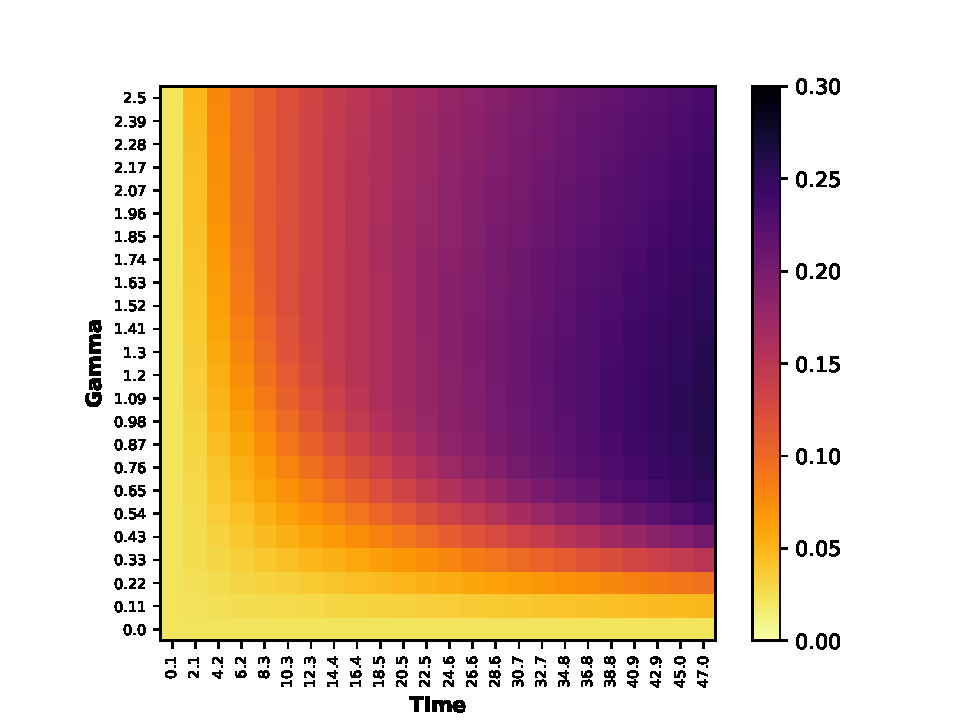
\includegraphics[width=75mm]{./figures/time_dependent_heatmap/47_heatmap_time_dependent_lin.pdf} &   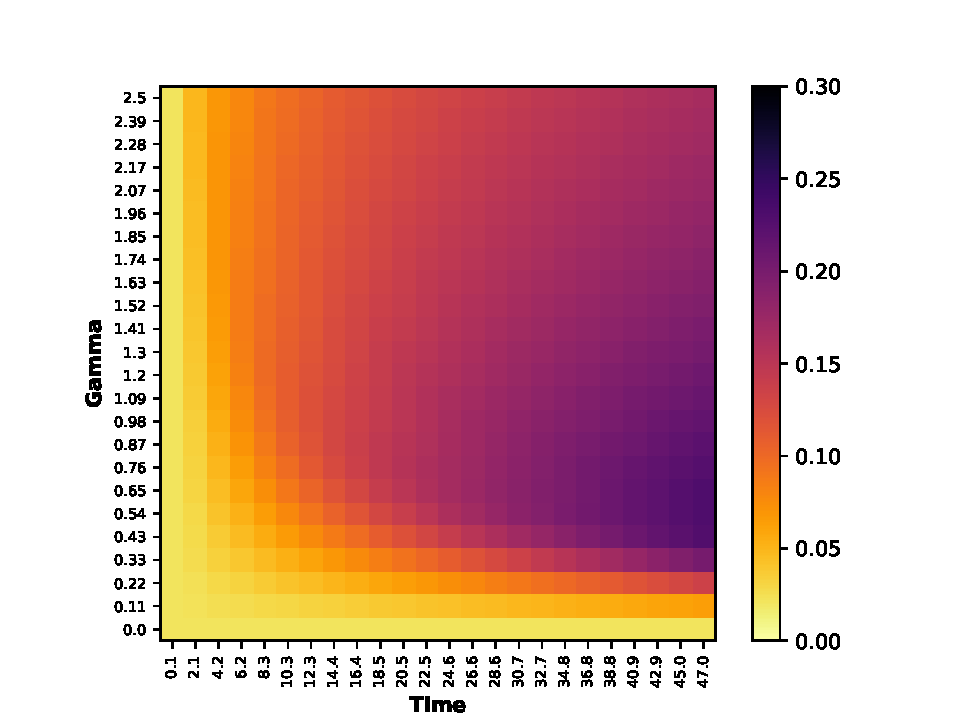
\includegraphics[width=75mm]{./figures/time_dependent_heatmap/47_heatmap_time_dependent_sqrt.pdf} \\
        (a) lin & (b) sqrt\\[6pt]
        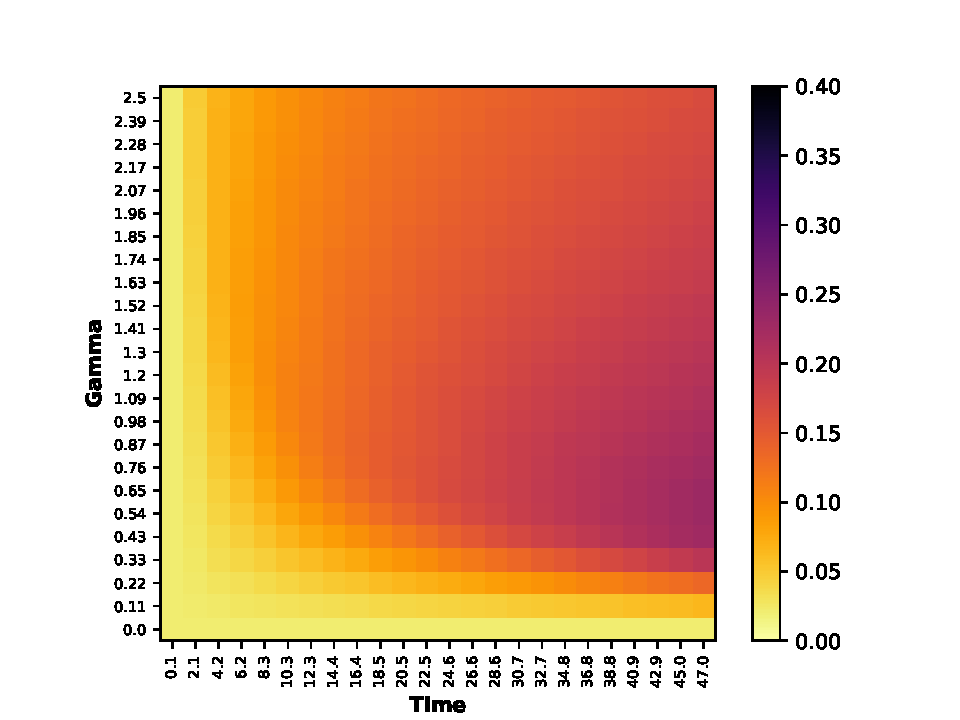
\includegraphics[width=75mm]{./figures/time_dependent_heatmap/47_heatmap_time_dependent_cbrt.pdf} &   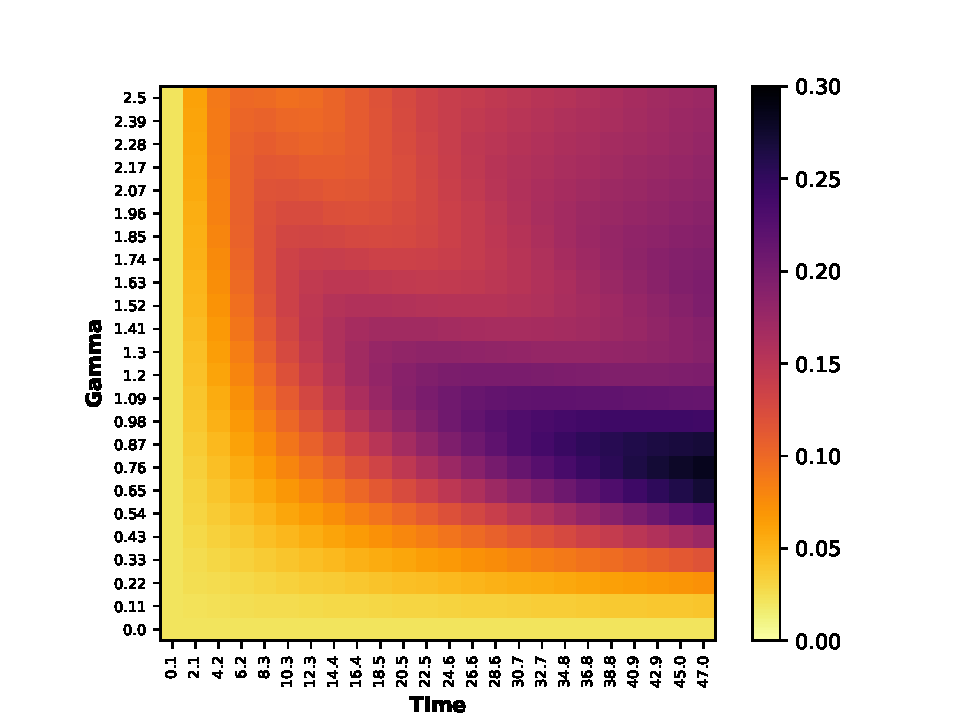
\includegraphics[width=75mm]{./figures/time_dependent_heatmap/47_heatmap_time_dependent_cerf.pdf} \\
        (c) cbrt & (d) cerf\\[6pt]
        \end{tabular}
        \caption[Probability heatmap plot for the time-dependent hamiltonian, for different shapes of s(t)]{\textbf{Probability heatmap plot for the time-dependent hamiltonian, for different shapes of s(t).} The figure shows the probability distribution for a circular graph of N=47 evaluated using the time-dependent hamiltonian using the following step functions (a) linear, (b) $\sqrt{t/T}$, (c) $\sqrt[3]{t/T}$ and (d) Ronald-Cerf(3). Note that the color gradient is normalized to p=0.3 to accentuate the difference in probability between different regions. }
        \label{time_dependent_heatmap}
        \end{figure}\\
        \subsubsection*{Comments on the probability distribution}
        Compared to the time-independent hamiltonain approach we can clearly see that the probability distribution is smoother (has no valley and peaks) both for constant $\gamma$ (any orizontal section) and constant $t_f$ (any vertical section). If we look at the different interpolating schedules it's immediately evident that the cbrt and sqrt schedules perform poorly compared to the linear one. On the other hand the Ronald-Cerf schedule performs in a similar way in terms of the highest probability found, but has a significantly different probability distributio, that might affect its robustness.
        \clearpage
    \subsection{Comparison: Localization}
        We now compare the localization properties of the two algorithm. As we mentioned in the comments to the probability distributions of the time-independent and time-dependent approaches we discovered the following:
        \begin{itemize}
            \item \textbf{Time-Independent QW}: the time-independent based search is not able to solve the search problem with a single iterations, thus making it necessary to run multiple searches. This implies that the approach does not show any localization properties, in fact the probability does not increase with time as in the time-dependent approach.
            \item \textbf{Time-Dependent QW}: the time-dependent based search on the other hand because of the adiabatic theorem does solve the search problem with a single iterations, although that happens for fairly large $t_f$.
        \end{itemize}
        Although the time-dependent approach is able to get to unitary probability in a fairly large $t_f$, it is able to produce large enough probabilities in much less time, as we can see from this plot. This is a consequence of the fact that the probability does not grow linearly with time, thus needing larger $t_f$ closer it gets to $P=1$. \textbf{A plot is needed}


    \subsection{Comparison: Search}
        In order to compare the two approaches for the search it is clear that we cannot simply consider the time at which the solution is found with unitary probability, since that particular $t_f$ is not optimized for the time-dependent approach and does not exist for the time-independent one. Therefore, as previously mentioned we consider the possibility of doing multiple runs for one search. For this reason we introduce the following quantity
        \begin{equation}
          \min\Big(\frac{t_f}{p}\Big)
        \end{equation}
        where $1/p$ is the number of iterations necessary to get to unitary probability (statistically), and combining it with $t_f$ gives the total time necessary. Optimizing over the combination of $t_f$ and $p$ gives the smallest time necessary to get to unitary probability using the multiple search approach. Additionally, the number of iterations $\mbox{iters}=1/P$ might give some useful insights on the performance of the approach, in particular if you take into account the initialization time $t_{init}$\\ \\  However, this particualar approach poses a few problems. Infact if we look at how the quantity $t_f/p$ varies for varying $t_f$, we discover that the minimum of such quantity will always be for the smallest $t_f$ available, regardless of the type of hamiltonian and step function $s(t)$. The following plot does indeed show, for a few sampled $\gamma$, the shape of $t_f/p$. In addition, in Section ? we mentioned that when dealing with multiple runs for one search we need to take into account an initialization time $t_{init}$. It is thus necessary to consider a lower bound on $t_f$.
        \begin{figure}[ht]
        \centering
        \begin{tabular}{cc}
          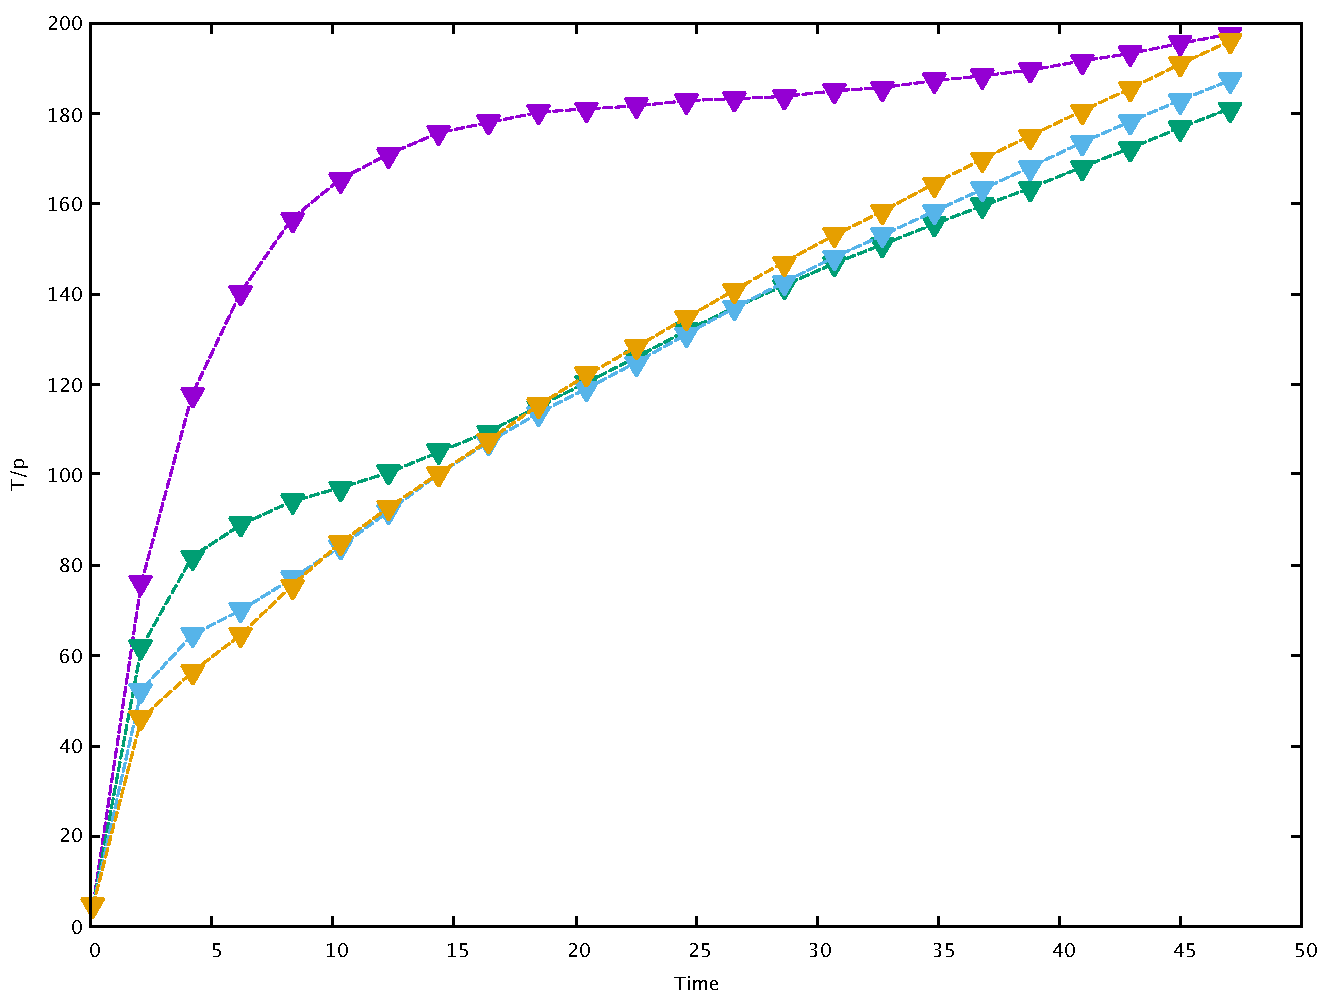
\includegraphics[width=75mm]{./figures/sampled_t_over_p/T_p_lin.pdf} &   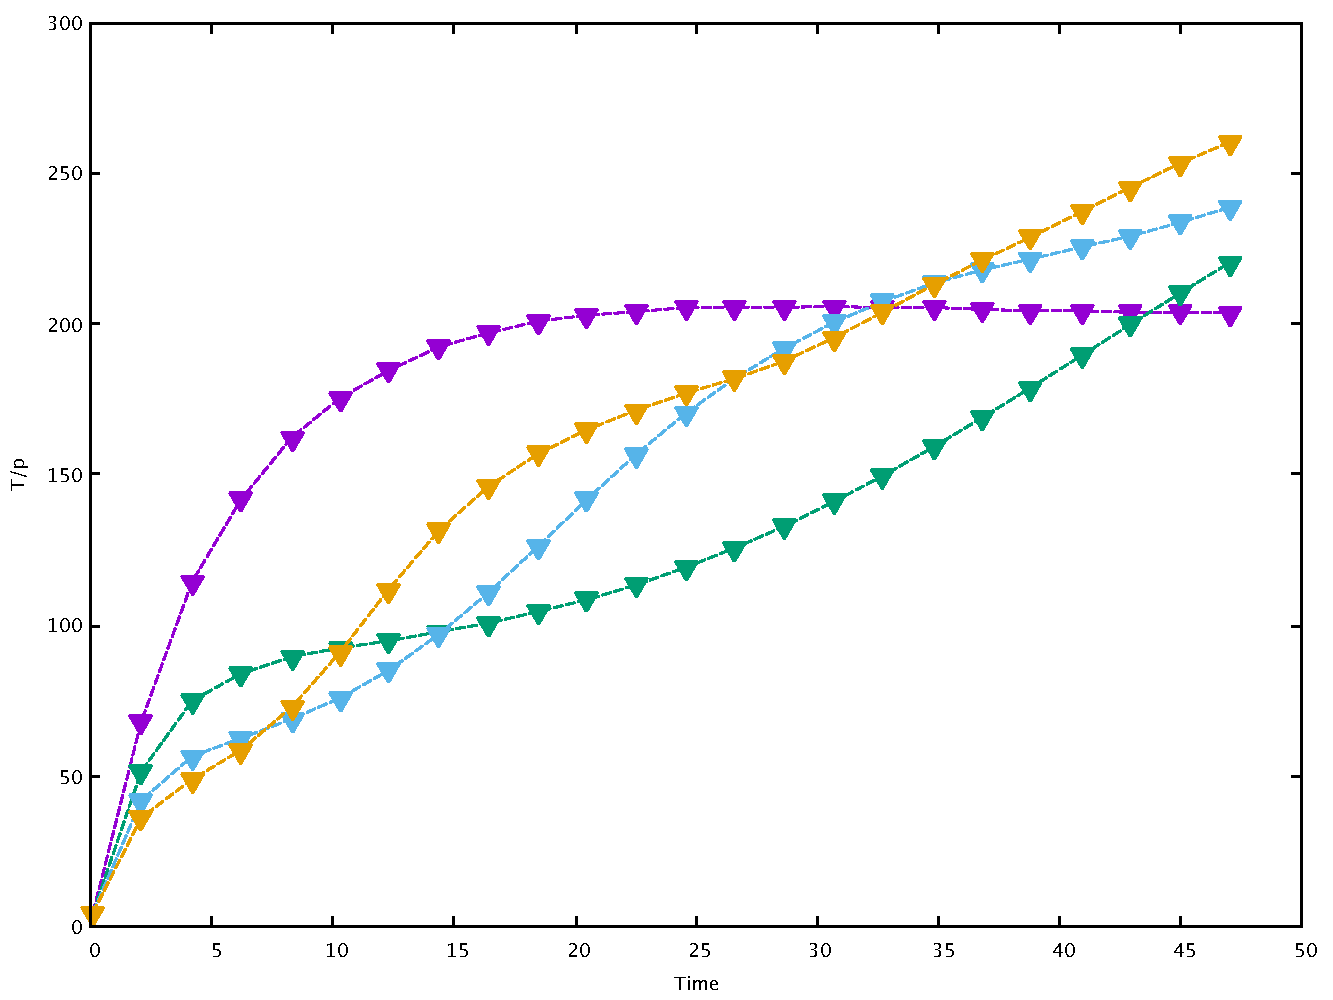
\includegraphics[width=75mm]{./figures/sampled_t_over_p/T_p_cerf.pdf} \\
        (a) lin & (b) Ronald-Cerf\\[6pt]
        \end{tabular}
        \caption[$t_f/p$ distribution for sampled $\gamma$ showing that the minimum will always be for the smallest $t$ ]{\textbf{Distribution of the quantity T/p for sampled $\gamma$ showing that tthe min(T/p) will always be the smallest for the smallest $t$.}he figure shows the distribution of the quantity $t_f/p$ for some sampled values of the parameter $\gamma$, using the linear and Ronald-Cerf interpolating schedules. It is clear that the quantity $\min(t_f/p)$ will always be for the smallest $t_f$ available, regardless of the interpolating schedule, requiring therfore a constrain on the time.}
        \end{figure}

        \bpar{\bm{$\min(t_f/p)$}  and run iterations for increasing lower bound \bm{$t_f$}}
         We will begin by studying how the quantity $\min(t_f/p)$ and $iters$ varies with increasing lower bound $t_f^*$.
         In the following plot we show the shape of $t_f/p$ with the time-independent approach and the time-dependent one; for the time being and for sake of semplicity, we consider only the step function Ronald-Cerf(3).
         \begin{figure}[h]
         \centering
         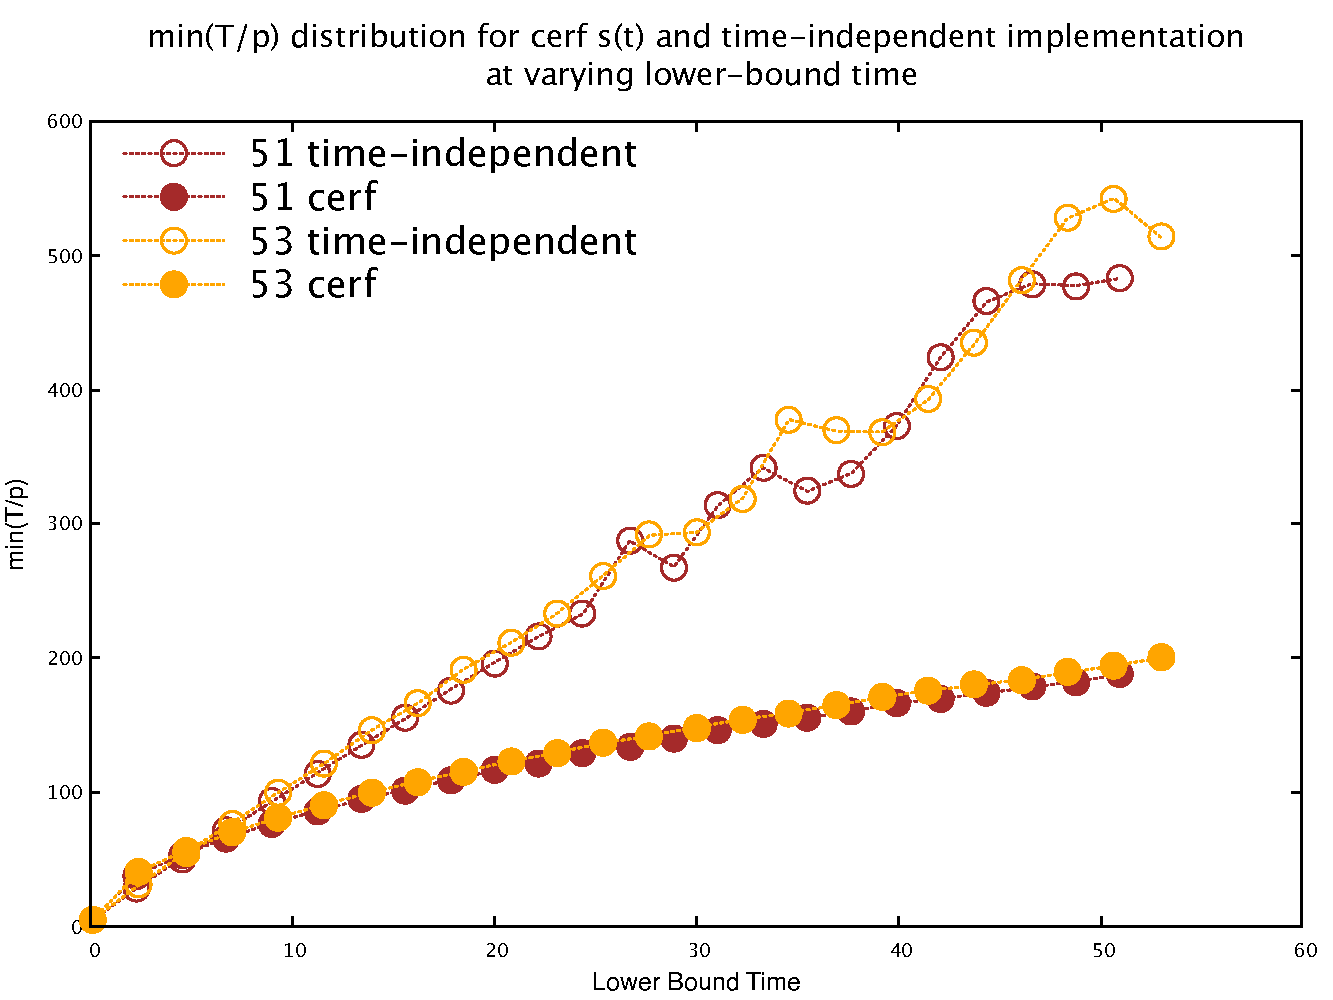
\includegraphics[width=80mm]{./figures/min_tp/delta.pdf}
         \caption[$\min(t_f/P)$ distribution for increasing lower bound time.]{\textbf{\bm{$\min(t_f/P)$} distribution for increasing lower bound time. }The figure shows the distribution of the quantity min(T/p) for increasing values of lower bound time, using the time-independent hamiltonian (circles) and time-dependent hamiltonain (solid circles) and evaluated for a Cy(51) and Cy(53). We see that for times smaller than a characteristic time $T^*$ the time-independent approach performs slightly better, while for large time the time-dependent one performs significantly better. }
         \label{fig:delta_increasing_time}
         \end{figure}
        As we can see from the plot the distribution can be diveded into to section marked by a particular $T^*$ (for the time being the value of such time is not of our interest):
        \begin{itemize}
            \item for $t_f<T^*$ the time-independent approach performes slightly better than the time-dependent one.
            \item for $t_f>T^*$ however the time-dependent approach performs significantly better, in particular with increasing time $t_f$
        \end{itemize}
        The behaviour for large T is to be expected, considering that the time-dependent approach shows localization properties and the probability increases with increasing time as we shoed in Figure?, in contrast with the time-independent approach that does not show localization propeties.\\ What this show is that the choice of $t_f$ has great effects on the outcome of our time-dependent approach, making it a successfull or unsuccesfull alternative.
        In terms of iterations the trend is similar to the quantity \quantity, as the following plot shows.
        \begin{figure}[ht]
        \centering
        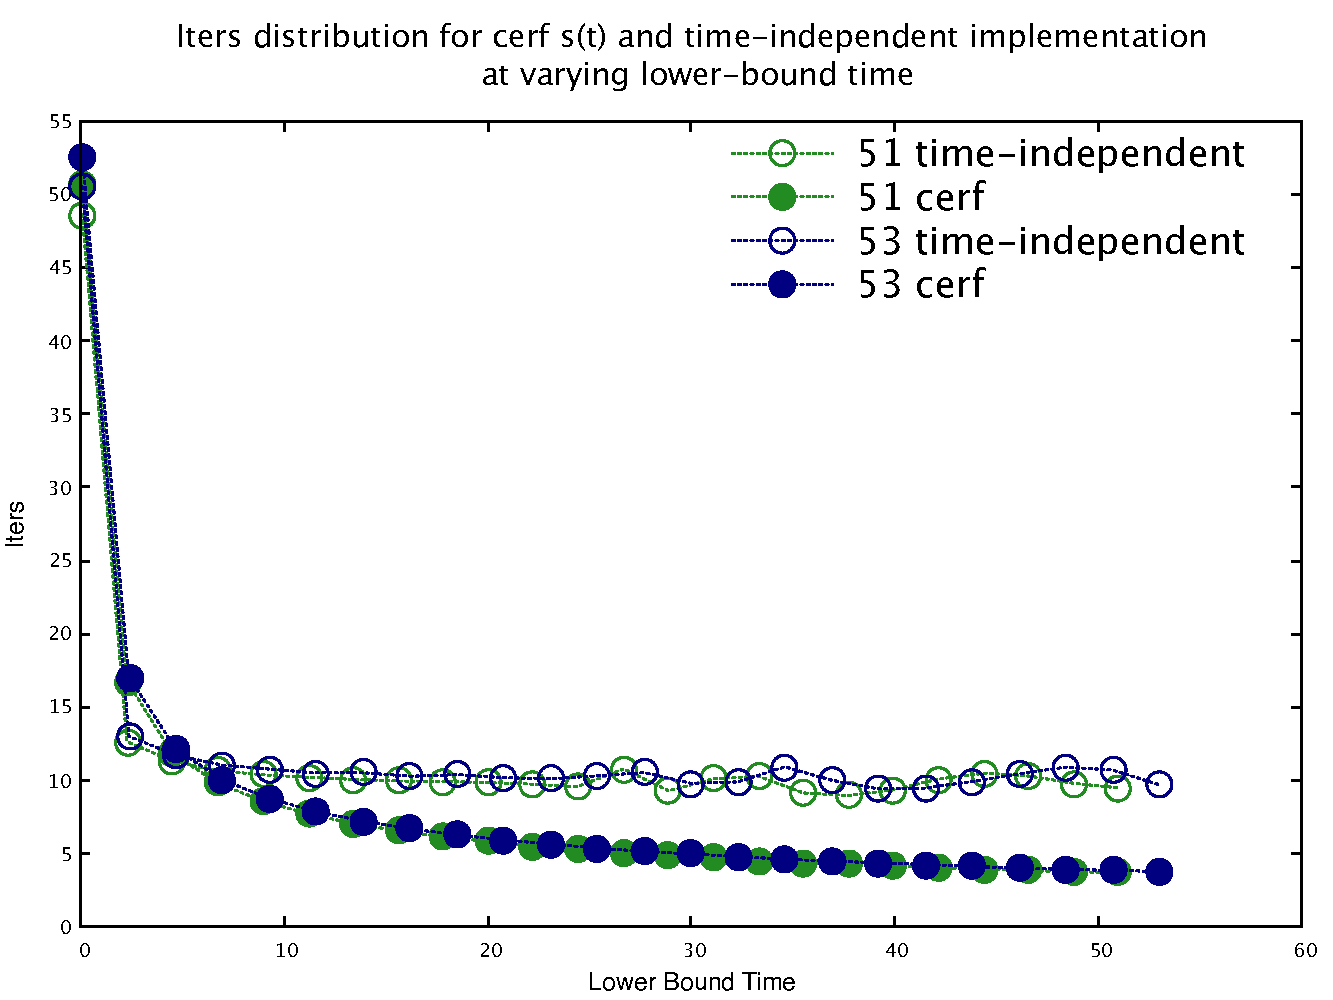
\includegraphics[width=90mm]{./figures/min_tp/iters.pdf}
        \caption[$iters$ distribution for increasing lower bound time.]{\textbf{$\bm{iters}$ distribution for increasing lower bound time. }The figure shows the distribution of $iters$ for increasing values of lower bound time, using the time-independent hamiltonian (circles) and time-dependent hamiltonain (solid circles) and evaluated for a Cy(51) and Cy(53). This distribution reflects the probability distribution of the two approaches: for the time-independent hamiltonian the probability does not increase with time, resulting in a (almost) constant $iters$, while the time-dependent hamiltonian showing localization properties requires less iterations to get to unitary probability.}
        \label{fig:iters_increasing_time}
        \end{figure} \\
        The iterations distribution reflects the overall probability distribution of the time-dependent and time-independent hamiltonian approaches. For small lower bound time the two approaches show a similar performance: the probability is very small, thus requiring a large number of iterations to get to unitary probability. As $t_f$ increases we see two very different trends:
        \begin{itemize}
            \item The time independent approach requires an almost constant number of iterations (the numerical values is somewhat irrelevant since this distribution reflects only the Cy(53) and Cy(55)). This reflects the non-localization properties of this particular approach, for which the probability does not increase with time
            \item On the other hand the time-dependent approach, showing localization properties, requires less iterations to solve the search with unitary probability.
        \end{itemize}
        Taking into account that we're performing a multiple run search and the initialization time $t_{init}$ previously discussed, it is clear that the time-depedent approch performs better than the time-independent counter part in most of the scenario.
        \clearpage
        \bpar{\bm{$\min(t_f/p)$} and run iterations with constrained lower bound time}
        In order to show that the lower bound time does indeed have such great impact on the performance of the time-dependen approach relative to the time-independent one we now study the distribution of the quantity $\min(t_f/P)$ with a constrain on the lower bound time. \\ The choice of constrain is arbitrary and somewhat biased since the larger the constrain the better the performance of the time-dependent approach, as we've just shown in \cref{fig:delta_increasing_time}. Therefore, to make the choice fair, we consider the lower bound time to be $t_f^* = 2\sqrt{N}$ which is (roughly) the time scaling of the standard Grover's Search, the QW Search on the complete graph and so on. In the best case scenario we discover that the number of iterations necessary to get to unitary probability remain constant regardless of the dimension of the graph, making this approach scale as the ones just mentioned; in the most probable scenario we discover that the number of iterations increase with the graph size, thus adding a scaling factor that depends on some power of N. \\ \\ The following plot shows the distribution of the quantity $\min(t_f/P)$ for circular graphs Cy(N) with N up to 71. The quantity is computed using the time-dependent hamiltonian with linear step function and the time-independent one, with constrained time $t_f=2 \sqrt{N}$.
        \begin{figure}[ht]
        \centering
        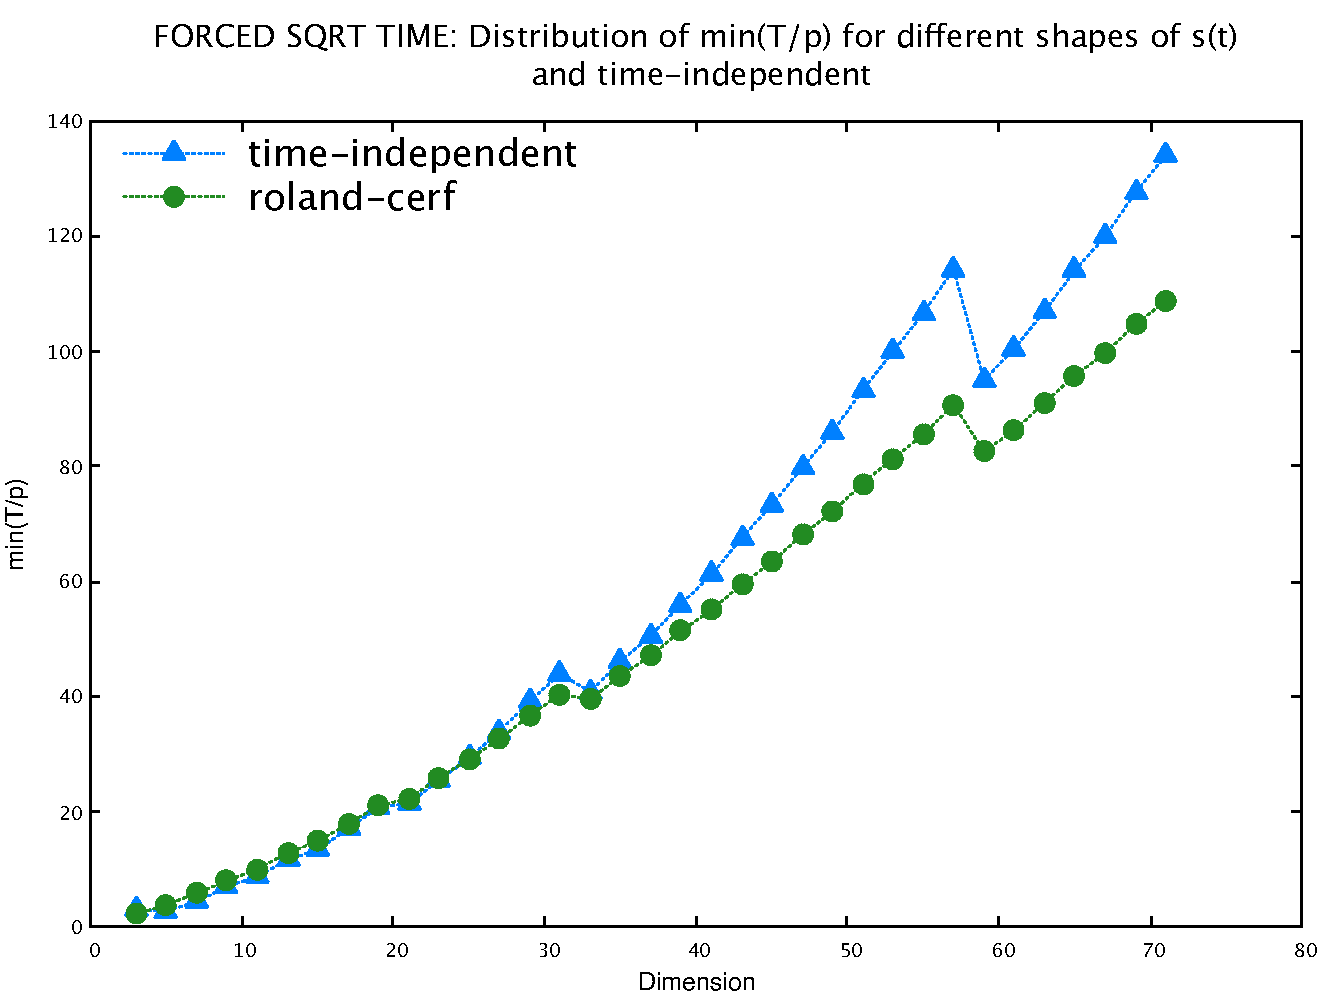
\includegraphics[width=80mm]{./figures/min_tp_sqrt/forced_delta.pdf}
        \caption[$\min(t_f/P)$ distribution for Cy(N) up to N=71 with constrained time at $\sqrt(N)$.]{\textbf{\bm{$\min(t_f/P)$} distribution for Cy(N) up to N=71 with constrained time at $\bm{2\sqrt{N}}$.} The figure shows the distribution of the quantity min(T/p) for increasing values of lower bound time, using the time-independent hamiltonian (circles) and time-dependent hamiltonain (solid circles) and evaluated for a Cy(51) and Cy(53). We see that for times smaller than a characteristic time $T^*$ the time-independent approach performs slightly better, while for large time the time-dependent one performs significantly better. }
        \label{fig:delta_increasing_time}
        \end{figure} \\ \\
        \bpar{\bm{$\min(t_f/p)$} and run iterations for different shapes of s(t)}
        We now investigate the effects of the different step functions discussed in section? in the probability distribution and in particular on the quantity $\min(t_f/P)$. As we did for the general time-dependent and time-independent comparison we constrain the lower bound time to be larger than $2\sqrt{N}$.
        The following plot shows the distribution of the quantity $\min(t_f/P)$ for circular graphs Cy(N) with N up to 71, using the time-dependent hamiltonian with linear, sqrt, cbrt and Ronald-Cerf(3) interpolating schedules $s(t)$:
        \begin{figure}[!h]
        \centering
        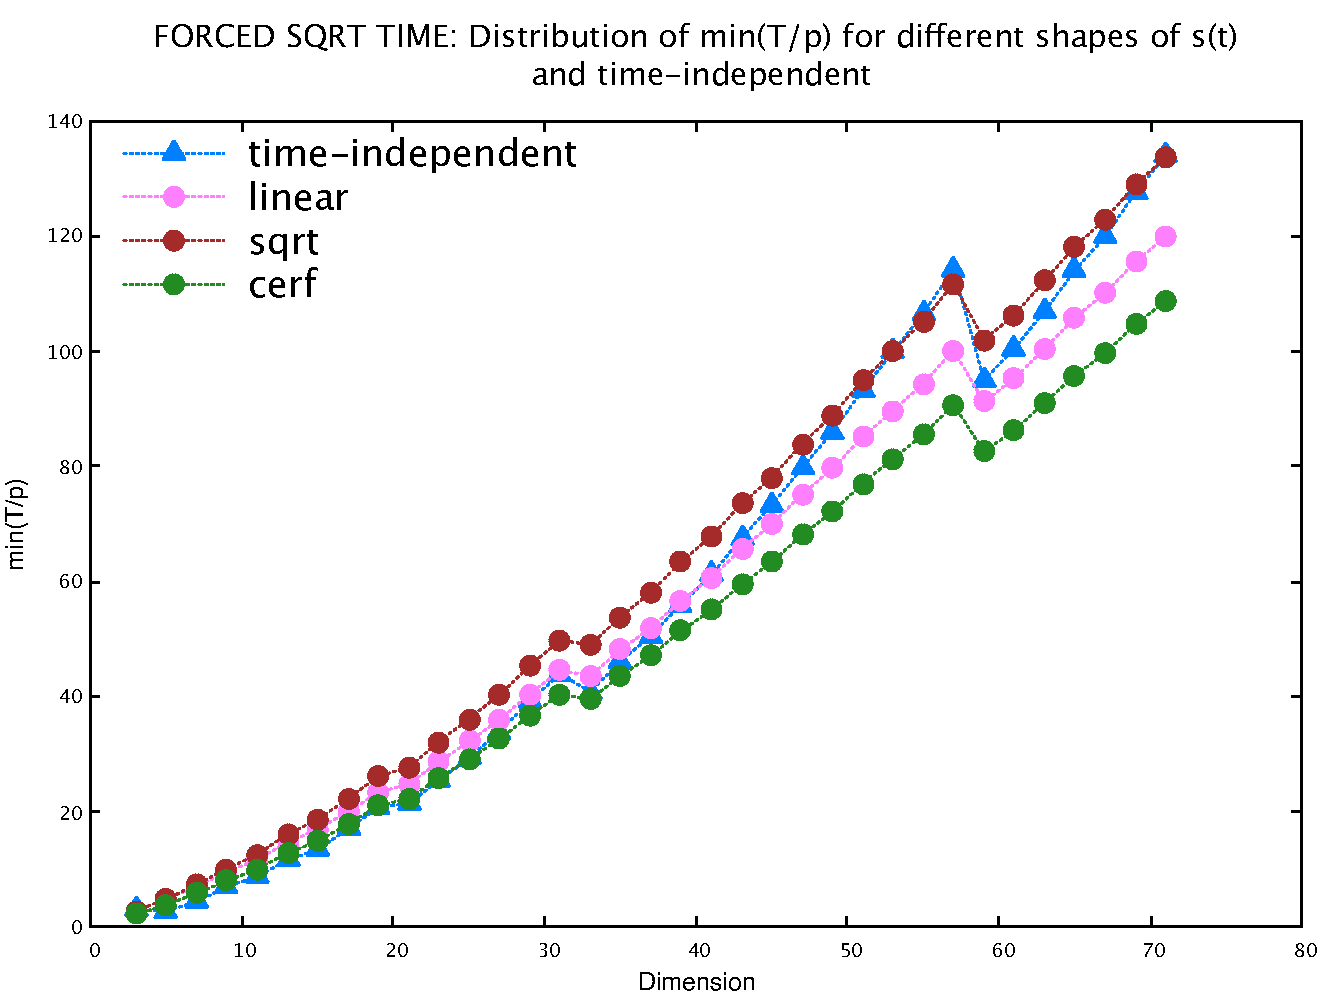
\includegraphics[width=80mm]{./figures/min_tp_sqrt/forced_sqrt_delta.pdf}
        \caption[$\min(t_f/P)$ distribution for Cy(N) up to N=71 with constrained time at $\sqrt(N)$ and different interpolating schedules.]{\textbf{\bm{$\min(t_f/P)$} distribution for Cy(N) up to N=71 with constrained time at $\bm{2\sqrt{N}}$ and different interpolating schedules.} The figure shows the distribution of the quantity min(T/p) with constrained lower bound time at $t_f= 2\sqrt{N}$, using the time-independent hamiltonian and time-dependent hamiltonain with different interpolating schedules. The abrupt changes are due to the resolution of the grid-probability evaluation (further discussions can be found in Appendix A)}
        \label{fig:delta_complete_sqrt}
        \end{figure}

        \noindent
        We can see from the plot that, as we might have expected, the Ronald-Cerf interpolating schedule performes better than the linear and sqrt schedules, in particular when we consider larger graph. For small enough N the time-independent approach performs slightly better, while for large N the time-depenedent approach is superior. Please note that the abrupt changes in the plot are due to the resolution of the grid-probability evaluation, discussed in Appendix A. \textit{nota: Additional computations will be run to try to fix this issue}.


    \subsection{Comparison: Robustness}
    We now address the robustness of the time-dependent and time-independent search. As we mentioned in Section? we're only interested in the comparison of the two approaches, and not an absolute measure of their robustness. Therefore we will use this measure solely as a comparison value. \\
    We proceed by considering small variations on the parameter $\gamma$ in the order of 1\% and 5\% (this numbers still need to be discussed). We begin by finding the quantity $\min(t_f/P)$ with time constrains ($t_f = 2\sqrt{N}$). For the corresponding $(t_f,\gamma)$ combination we evaluate the robustness R as defined in Section?
    For the time-dependent search with only consider the linear step function an the Ronal-Cerf(3). As we showed in the previous section the Ronald-Cerf Hamiltonian performs better than the linear conterpart, while from a qualitative point of view the linear hamiltonian has a smoother probability distribution (see \cref{time_dependent_heatmap}(a)-(d)). The following plots show the semi-quantitative robustness for the $\gamma$ variations in the order of 1\% - 5\% for the time-independent search and the time-dependent one with linear and Ronald-Cerf step functions s(t). \textbf{Computations are still needed}

    %ROBUSTNESS PLOT
    %%
%PROBABILITY DISTRIBUTION FOR SAMPLED N, UP TO P=1
%%

\begin{figure}[ht]
\centering
  \begin{tikzpicture}
    \begin{axis}[name=plot
    xmin=0, xmax=441,
    ymin=0, ymax=1,
    width = 120mm,
    height=95mm,
    xlabel = $\bm{T}$,
    ylabel = $\bm{p}$,
    legend style={at={(0.95,0.05)},
    anchor=south east}]
    \addplot[color=verdescuro,no marks, thick, x=a, y=b] table{./Data/fig6/fig6_21_lin.txt};\addlegendentry{$N=21$, $\gamma=1.5$, $s_L(t)$}
    \addplot[color=verdescuro,dashed, no marks, thick, x=a, y=b] table{./Data/fig6/fig6_21_cerf.txt};\addlegendentry{$N=21$, $\gamma=1.05$, $s_{RC}(t)$}

    \end{axis}
  \end{tikzpicture}
  \caption{\textbf{Probability distibution for a $\bm{Cy(21)}$ with sampled $\bm{\gamma}$}: The figure shows the probability distribution for the cycle graph $Cy(21)$, evaluated with the time-dependent hamiltonian using the interpolating schedules (solid) linear $s_L$ and (dashed) Roland-Cerf $S_{RC}$. We can see that the probability increases with time, as expected. }
  \label{fig:probability_sampled_gamma}
\end{figure}



\section{Results for the Complete Graph}
    \subsection{Search results from Wong(2016)}
    \subsection{Localization results}

%\section{Results for the complete graph}
We now turn our attention to the complete graph. As we discussed in the preliminaries in \Cref{subsec:search qw complete graph} and \Cref{subsec:local adiabatic}, with the complete graph we are able to solve the search problem using the standard time-independendent quantum walks Hamiltonian with time scaling of $O(\sqrt{N})$. Additionally for the unstructured search - which is equivalent to a search on the complete graph - we showed that with the local adiabatic evolution it is possible to get the same speedup of $O(\sqrt{N})$, while that was not the case for the global adiabatic evolution that had the same time scaling as the classical search. Although Wong proved that for the complete graph it is not possible to solve the search problem with an adiabatic quantum walk algorithm, for completeness we extend the time-dependent Hamiltonian implementation to the complete graph. Clearly we are not able to achieve any speedup nor necessarily any comparable time scaling, but we might get some interesting insights in terms of probability distribution and robustness.

    \subsection{Comments on the placement of $\gamma$}
    Firstly we recall that in \Cref{subsec:complete graph} we introduced the search Hamiltonian as
    \begin{equation}
      H = \gamma L -\ket{w}\bra{w}
    \end{equation}
    We quickly notice that the $\gamma$ parameter is in front of the Laplacian, compared to the time-dependent Hamiltonian considered throughout our work where $\gamma$ was placed in front of the oracle $\ket{w}\bra{w}$. We could now proceed by comparing the time-independent and time-dependent approaches with the $\gamma$ placement as in literature - i.e. in front of the Laplacian - or as we did in \Cref{sec:time_dependent_Hamiltonian}. In order to be consistent with the standard quantum walks search on the complete graph discussed in \Cref{subsec:search qw complete graph} we proceed by considering the following Hamiltonians, with $\gamma$ in front of the Laplacian. This ensures that the time-dependent probability distribution is compatible with the time-independent one, and does not require to re-evaluate the optimal $\gamma$ for the time-independent approach. Nevertheless the two approaches can be considered equivalent. The Hamiltonians are given by
    \begin{equation}
      H = \gamma L-\ket{w}\bra{w}\hspace{45pt}\mbox{(independent)}
    \end{equation}
    \vspace{-0.5cm}
    \begin{equation}
      H(s) = (1-s)\gamma L - s\ket{w}\bra{w}\hspace{20pt}\mbox{(dependent)}
    \end{equation}\\


    \noindent
    Having defined the Hamiltonians, we proceed as in the previous section, following however a more qualitative approach. In order to do so we compare the probability distribution using the heatmap plots introduced in \Cref{subsec:time_independent_benchmarks, subsec:time_dependent_results}.


    \subsection{Probability distribution and qualitative robustness}
    Recalling that for the time-independent quantum walks implementation the optimal $\gamma$ is given by $\gamma=1/N$, we evaluate the probability for $\gamma$ in a neighbourhood of $1/N$ and up to $T=N$. This allows us to have a complete picture of the probability distribution, as can be seen in the following heatmap plots.

    %%
%COMPLETE GRAPH LOCALIZATION HEATMAP
%%

    As previously discussed we are able to solve the search problem with the time-independent algorithm in a time of the order of $T=\pi/2\sqrt{N}$. Indeed we see from the figure above that the probability is close to $p=1$ for $T=11$, as expected. On the other hand the time-dependent approach is able to solve the search with a single iteration for $T\rightarrow N$, showing no significant speedup compared to the classical search. This however leaves space for a multiple run search as introduced in \Cref{subsec:multiple_runs}. We therefore investigate this possibility by evaluating the maximum probability found for $T=\pi/2\sqrt{N}$ with the time-dependent algorithm and study the \textbf{iterations} distribution.

    %%
%T - ROBUSTNESS
%%
\begin{figure}[ht]
  \centering
  \begin{tikzpicture}

    \begin{axis}[name=plot,
    xmin=0, xmax=110,
    ymin=0, ymax=7,
    width = 100mm,
    xlabel = Dimension $N$,
    ylabel = Iterations $I$]
    \addplot[color=rossoscuro,mark=*,mark size=2.5pt, x=a, y=b] table{./Data/fig18/iterations.txt};\addlegendentry{iterations}
    \end{axis}\label{plot_one}

    \begin{axis}[name=plot,
    axis y line*=right,
    axis x line=none,
    xmin=0, xmax=110,
    ymin=0, ymax=1,
    width = 100mm,
    xlabel = Dimension $N$,
    ylabel = Probability $p$]
    \addlegendimage{mark=*,mark size=2.5pt, color=rossoscuro}\addlegendentry{Iterations}
    \addplot[color=verdescuro,mark=*,mark size=2.5pt, x=a, y=b] table{./Data/fig18/probability.txt};\addlegendentry{Probability}

    \end{axis}


  \end{tikzpicture}
  \caption[]{\textbf{Iterations \bm{$I$} and probability \bm{$p$} for the multiple run search on complete graph.} The plot shows the probability $p$ and the number of iterations $I$ for the multiple run search with the time-dependent Hamiltonian. The time is constrained to $\pi/2\sqrt{N}$ as in the solution of the standard quantum walks search. It is clear that the number of iterations increases linearly, although very slowly. Notice in fact that $N$ goes all the way up to $N=101$. For the limit of large $N$ the time-dependent approach is therefore not a valid alternative, nor of comparable performance.}
  \label{fig:iterations_complete_graph}
\end{figure}


    It is clear from the plot that the number of run iterations increases with the graph size linearly, although very slowly (notice that $N$ goes up to 101). In the limit for large $N$ the multiple runs search does not improve the time-dependent approach, therefore the standard quantum walks search remains the strongest option.
    \\


    \noindent
    However, we can now address the \textbf{robustness} properties of the two approaches. Similarly to the cycle graph, the complete graph has a probability distribution with regions of high and low probability when considering the time-independent Hamiltonian. Compared to the smooth probability distribution of the time-dependent algorithm we can safely say that the latter is more robust than the first, both for noise on $T$ and $\gamma$. It is to be noted however that for the cycle graph the time-independent and time-dependent approaches are of comparable performance, therefore the robustness has a great impact to the overall performance. In this scenario the time-independent approach performs better in terms of probability, and having less robustness does not justify the \textit{almost} linear time-scaling of the time-dependent one. \\


    \noindent
    Although the time-dependent algorithm is not able to perform as well as the time-independent one, striking is the difference in probability distribution between the non-linear $s_{NL}(t)$ and the linear $s_L(t)$, showing the importance of the shape of the interpolating schedule. From the following plots we can see that the time-dependent Hamiltonian with the linear interpolating schedule $s_L(t)$ is not able to solve the search for $T=N$. The improvement on the performance is therefore achieved by findind the optimal interpolating schedule.

    %%
%COMPLETE GRAPH HEATMAP PLOTS - ROLAND-CERF and LINEAR
%%

\begin{figure}[ht]
  \centering
  \subfloat[][$s_{NL}(t)$]
  {
    \hspace{-0.8cm}
    \begin{tikzpicture}
      \begin{axis}[name=plot,
      zmin=0,zmax=1,
      view={0}{90},
      colormap={inferno}{rgb255=(248,251,155) rgb255=(251,179,21) rgb255=(236,103,38) rgb255=(187,54,84) rgb255=(119,29,109) rgb255=(49,9,92) rgb255=(1,1,8)},
      colorbar,
      colorbar right,
      point meta min=0,
      point meta max=1,
      width = 65mm,
      height= 65mm,
      xlabel = $\bm{T}$,
      ylabel = $\bm{\gamma}$
      ]
      \addplot3 [surf] table[x=a,y=b,z=c]{./Data/fig17/51_cerf_complete.txt};

      \end{axis}
    \end{tikzpicture}
  }
  \subfloat[][$s_L(t)$]
  {
    \begin{tikzpicture}
      \begin{axis}[name=plot,
      zmin=0,zmax=1,
      view={0}{90},
      colormap={inferno}{rgb255=(248,251,155) rgb255=(251,179,21) rgb255=(236,103,38) rgb255=(187,54,84) rgb255=(119,29,109) rgb255=(49,9,92) rgb255=(1,1,8)},
      point meta min=0,
      point meta max=1,
      width = 65mm,
      height= 65mm,
      xlabel = $\bm{T}$,
      ylabel = $\bm{\gamma}$,
      ylabel near ticks, yticklabel pos=right
      ]
      \addplot3 [surf] table[x=a,y=b,z=c]{./Data/fig17/51_linear_complete.txt};
      \pgfplotsset{contour/every contour label/.style = {
                 sloped,
                 inner sep=2pt,
                 transform shape,
                 every node/.style={mapped color,fill=none},
                },}
      \addplot3[
              contour gnuplot=
              {
              draw color=white,
              levels={0.5},
              labels=true,
              contour label style={nodes={text=white,font={\large}, yshift=-2.5ex, xshift=3.0ex}},
              handler/.style=smooth},
              contour/label distance=300pt,
              line width=1.5pt,
              contour/labels over line
             ] table [
                      x = a,
                      y = b,
                      z = c,
                     ]{./Data/fig17/51_linear_complete.txt};
      \end{axis}
    \end{tikzpicture}
  }

  \caption[]{\textbf{Probability distributions for the complete graph \bm{$C(51)$} with the time-dependent Hamiltonian.} The figure shows the probability distribution for a complete graph of $N=51$ using the time-dependent Hamiltonian with the non-linear $s_{NL}(t)$ (a) and linear $s_L(t)$ (right) interpolating schedules. It illustrates the great impact of the interpolating schedule on the overall performance of the time-dependent algorithm, where the choice of $s(t)$ is critical.}
  \label{fig:heatmap-complete}
\end{figure}


%%%%%%%%%%%%%%%%%%%%%%
%%%%%%%%%%CONCLUSIONS%%%%%%%
%%%%%%%%%%%%%%%%%%%%%%%
\newpage


\chapter*{\textbf{Conclusions}}
\addcontentsline{toc}{chapter}{Conclusions}

\vspace{-1cm}
We conclude our work with a summary of what has been accomplished in this thesis, some thoughts on the results and future perspective. \\

In Chapter 1 we reviewed some basic notion of graph theory, quantum walks, and the main characteristics of the graph topologies considered. We then introduced the search problem as originally posed by Grover - with particular enphasis on the action of the \textit{oracle} - followed by its quantum walks implementation of Farhi and Gutmann on the complete graph. We then discussed the adiabatic theorem and its application to the search problem, focusing on the difference between the global and local adiabatic evolution. To set the basis for our work we presented the work by Wong et. al \cite{Wong2016}, where they show that an adiabatic-quantum walk implementation of the search algorithm is not possible with the structure of the standard Grover's oracle. \\

In Chapter 2 we introduced the main topic of our work which is a quantum walks search algorithm with time-dependent Hamiltonians, \textit{inspired} by the adiabatic implementation but free of the constrains of the adiabatic theorem. We introduced a few classes of interpolating schedules with the goal of improving the standard linear one of Farhi and Gutmann. We draw from the one derived by Roland and Cerf, and consider the following non-linear interpolating schedule:
\begin{equation*}
  s_{NL}(t)  = \frac{1}{2}\Big[\big(2\frac{t}{T} - 1\big)^3 +1\Big].
\end{equation*}
Additionally we also consider the possibility of repeating the search multiple times if the search is not perfect - that made us take into account an initialization and measure time. In order to compare the time-independent and time-dependent approach we introduced three classes of results: the search, the localization and the robustness. \\

We then turned our attention to the cycle graph, the main graph topology considered. We studied the localization, search and robustness. \\
In terms of localization we discovered that the probability evaluated with the time-independent Hamiltonian does not increase with time, therefore it does not show localization properties. On the other hand, the time-dependent approach - given that it based on the adiabatic implementation - for large $T$ (far larger than the classical $O(N)$ search) it is able to achieve unitary probability. More interestingly, since the probability does not increase linearly, the solution of the search can be found with probability in the order of $p=0.8\div 0.9$ in much less time. \\

\noindent
We then studied the search performance of the two approaches in terms of multiple runs search. Therefore we introduced a new quantity which represents the minimum time necessary to get to unitary probability:
\begin{equation*}
  \tau = \min\Big(\frac{T}{p}\Big)_{T,\gamma}.
\end{equation*}
We also consider the number of run iterations $I=\min(p^{-1})_{T,\gamma}$. Additionally we discover that $\tau$ requires to consider a minimum time $T_{\min}$ to be effective at comparing the two approaches. To be consistent with the standar Grover's and the quantum walks search we set $T_{\min} = \pi/2\sqrt{N}$. \\
After seeing that for the time-dependent approach the linear and non-linear interpolating schedules $s_L$ and $s_{NL}$ perform the best, we compare them to the time-independent approach.\\
We discovered that both approaches have similar performance up to $N\approx 25$, while for large $N$ it gets significanly different, with the $s_{NL}$ performing the best and the time-independent approach the worst. In terms of run interations $I$ we see that the time-dependent approach, regardless of the interpolating schedules, performs better than the classical search, but still much worse than the optimal time scaling of $O(\sqrt{N})$. Although promising, this result is limited to the dimension considered - up to $N=71$ in our analysis - and therefore cannot be generalized for large $N$. \\

\noindent
We then studied the robustness for both time and $\gamma$. The time-independent approach has a very discontinous probability, made of scattered regions of high and low probability, leading to being less $\gamma$-robust than the time-dependent approach. Indeed the latter has a smooth probability distribution regardless of the interpolating schedule considered. Nevertheless the linear $s_L$ leads to more robust results than $s_{NL}$. In terms of $T$-robustness the time-independent approach is surprisingly more robust than the others, although the difference in robustness is much smaller than the one encountered for the $\gamma$-robustness. Therefore we can safely say that the time-dependent Hamiltonian-based algorithm is more robust than the time-independent one. \\


For completeness we at last turned our attention to the complete graph, qualitatively comparing the probability distribution and the robustness. As expected the time-dependent approach is not able to achieve comparable performance with the standard time-independent algorithm.  In terms of qualitative robustness we see that the time-dependent algorithm has a smoother probability distribution and therefore better robustness. However the improvement in robustness does not justify the much worse time scaling. \\
The complete graph however illustrates the importance of the interpolating schedule. In particular, with the time-dependent approach and linear $s_L$ the maximum probability reached is $p=0.5$ in  $T=N$ for a $C(51)$. With the improved non-linear interpolating schedule $s_{NL}$ we're able to achieve in $T=N$ a maximum probability of $p>0.9$.\\


Although it is not able to acheive the same time scaling as the time-independent approach it suggests that the improvement on performance comes from the choice of the optimal interpolating schedule. Future investigation on the interpolating schedule is necessary to 


%%%%%%%%%%%%%%%%%%%%%%
%%%%%%%%%%APPENDIX%%%%%%%
%%%%%%%%%%%%%%%%%%%%%%%
%\newpage
\chapter*{Appendices}
\addcontentsline{toc}{chapter}{Appendices}
\phantomsection
\section*{Appendix A: Probability Grid Evaluation}
\addcontentsline{toc}{section}{Appendix A: Probability Grid Evaluation}
\phantomsection
\section*{Appendix B: Computational Routines}
In this section an overview of the computational methods is presented, focusing the attention on the \textbf{optimization algorithm} and the \textbf{differential equation solver}. Additionally the normalization error is discussed. Lastly computational reasoning for the \textbf{probability grid evaluation} are presented. \\

Most all numerical simulations were performed using \textbf{Python}. Numerical methods such as optimization and ODE Solver come directly from python's native \textbf{Scipy}. In addition, a CPU-multiprocessing library, \textbf{Ray}, has been used to speed up the grid probability evaluation quite noticeably. Heatmap plots were created using python matplotlib, while additional plots were created with gnuplot.

\subsection{Optimization Algorithm}
In Section III a series of benchmark were performed to compare the time-dependent and time independent hamiltonian approach to the search problem. In order to determine which optimization algorithm fitted the best for the task, a number of possible algorithm were tested, such as \textit{shgo, dualannealing, minimize, LHSBH} and \textit{Basin-Hopping}.\\ \\
Due to the oscillating nature of the probability (\red{a figure is needed}) the scipy native \textbf{Basinhopping algorithm} was used. As the name suggests the algorithm performs a series of randomized hops, i.e. jumps, of the coordinates in order to find the true maximum This fits particularly well with the series of maxima and minima of the probability function (for fixed $\gamma$) in the time-independent hamiltonian. \\\red{Additional information on the parameter used are needed (e.g. step size, number of iterations)}

\subsection{Schroedinger Solver and Normalization Error}
In Section II we presented an evolution which is governed by a time-dependent hamiltonian, used to find the evolved state $|\psi(t)\rangle$. This is accomplished by solving the usual Schroedinger equation using Scipy's \textbf{integrate.solve\_ivp}, that provides a wide varieties of integrations methods. \\

As it's routine we used Runge-Kutta RK45, which as stated in the documentation it's a explicit Runge Kutta method of order 4(5). The error is controlled assuming fourth order accuracy, but steps are taken using the fifth-order accurate formula. In addition, the integrator is adaptive, meaning that the time step is chosen for optimal error control. Regarding the error, the algorithm provides two distinct parameters to set a targeted limit, namely the \textbf{relative (rtol)} and \textbf{absolute tolerances (atol)}. The first provides a relative accuracy, i.e. the number of digits, while the latter is used to keep the local error estimate below the threshold \textit{atol + rtol*abs(y)}. Determining the correct combinations of the two parameters is key for achieving the desired error. A few of those are presented in the following table, where a worst case scenario (N=101, T=1000) is used and the error is evaluated on the expected normalized state. The combination of rtol and atol bolded is the one we used in the solver, which gives us a small enough error on the normalization without greater computational expense.\\
\addcontentsline{toc}{section}{Appendix B: Computational Routines}

%%%%%%%%%%%%%%%%%%%%%%
%%%%%%%%%%BIBLIOGRAPHY%%%%%%%
%%%%%%%%%%%%%%%%%%%%%%%
%\newpage
%\chapter*{Bibliography}
\bibliography{bibliography/my_library}{}
\bibliographystyle{abbrv}
\addcontentsline{toc}{chapter}{Bibliography}


\end{document}
